
\documentclass[12pt, a4paper]{report}
\usepackage{epsfig}
\usepackage{subfigure}
%\usepackage{amscd}
\usepackage{amssymb}
\usepackage{graphicx}
%\usepackage{amscd}
\usepackage{amssymb}
\usepackage{subfiles}
\usepackage{framed}
\usepackage{subfiles}
\usepackage{amsthm, amsmath}
\usepackage{amsbsy}
\usepackage{framed}
\usepackage[usenames]{color}
\usepackage{listings}
\lstset{% general command to set parameter(s)
basicstyle=\small, % print whole listing small
keywordstyle=\color{red}\itshape,
% underlined bold black keywords
commentstyle=\color{blue}, % white comments
stringstyle=\ttfamily, % typewriter type for strings
showstringspaces=false,
numbers=left, numberstyle=\tiny, stepnumber=1, numbersep=5pt, %
frame=shadowbox,
rulesepcolor=\color{black},
,columns=fullflexible
} %
%\usepackage[dvips]{graphicx}
\usepackage{natbib}
\bibliographystyle{chicago}
\usepackage{vmargin}
% left top textwidth textheight headheight
% headsep footheight footskip
\setmargins{3.0cm}{2.5cm}{15.5 cm}{22cm}{0.5cm}{0cm}{1cm}{1cm}
\renewcommand{\baselinestretch}{1.5}
\pagenumbering{arabic}
\theoremstyle{plain}
\newtheorem{theorem}{Theorem}[section]
\newtheorem{corollary}[theorem]{Corollary}
\newtheorem{ill}[theorem]{Example}
\newtheorem{lemma}[theorem]{Lemma}
\newtheorem{proposition}[theorem]{Proposition}
\newtheorem{conjecture}[theorem]{Conjecture}
\newtheorem{axiom}{Axiom}
\theoremstyle{definition}
\newtheorem{definition}{Definition}[section]
\newtheorem{notation}{Notation}
\theoremstyle{remark}
\newtheorem{remark}{Remark}[section]
\newtheorem{example}{Example}[section]
\renewcommand{\thenotation}{}
\renewcommand{\thetable}{\thesection.\arabic{table}}
\renewcommand{\thefigure}{\thesection.\arabic{figure}}
\title{Research notes: linear mixed effects models}
\author{ } \date{ }


\begin{document}
\author{Kevin O'Brien}
\title{Mixed Models for Method Comparison Studies}
\tableofcontents

%----------------------------------------------------------------------------------------%
\newpage






	\chapter{Residual and Influence Diagnostics}
	\section{Chapter Overview}
	\begin{enumerate}
		\item Residual Diagnostics
		\begin{enumerate}
			\item Marginal and Conditional Diagnostics
			\item Scaled Residuals
		\end{enumerate}
		
		\item Influence Diagnostics
		\begin{enumerate}
			\item Underlying Concepts
			\item Managing the Covariance Parameters
			\item Predicted Values, PRESS Residual and the PRESS Statistic
			\item Leverage
			\item Internally and Externally Studentized Residuals
			\item DFFITs and MDFFITs
			\item Covariance Ratio and Trace
			\item Likelihood Distance
			\item Non-iterative Update Procedures
		\end{enumerate}
	\end{enumerate}
	\newpage
	%-----------------------------------------------------------------------------------------%
	\section{Residual Diagnostics}
	
	Consider a residual vector of the form $\hat{e} = \boldsymbol{PY} $, where $\boldsymbol{P}$ is a projection matrix, possibly an oblique projector.
	External studentization uses an estimate of $Var$ that does not involve the $i$th observation.
	Externally studentized residuals are often preferred over studentized residuals because they have well known distributional
	properties in the standard linear models for independent data.
	Residuals that are scaled by the estimated variances of the responses are referred to as Pearson-type residuals.
	Standardization: \[ \frac{\hat{e}_i}{\sqrt{v_i}}\]
	Studentization \[ \frac{\hat{e}_i}{\sqrt{\hat{v}_i}}\]
	
	\subsection{Introduction}
	\subsection{Marginal and Conditional Diagnostics}
	[Gregoire,Schabenberger, Barrett (1995)]
	
	\[\boldsymbol{r}_{m} = \boldsymbol{Y} -  \boldsymbol{X} \boldsymbol{\hat{\beta}} \]
	
	\[\boldsymbol{r}_{c} = \boldsymbol{Y} -  \boldsymbol{X} \boldsymbol{\hat{\beta}} -  \boldsymbol{Z} \boldsymbol{\hat{\gamma}}\]
	
	For the individual observation the raw studentized and pearson type residuals are computed as follows:
	\[r_{mi} =Y_{i} -X^{\prime} \boldsymbol{\hat{\beta}}\]
	
	\[r_{ci} = r_{mi} - Y_{i} - z_{i}^{\prime} \boldsymbol{\hat{\gamma}}\]
	
	%------------------------------------------------------------Section 4.1---%
	\subsubsection{Marginal Residuals}
	The marginal residuals are defined according to
	\begin{eqnarray*}
		\hat{\xi} = y - X\hat{\beta} = M^{-1}Qy. \\\nonumber
	\end{eqnarray*}
	
	Plots of the elements of the marginal residual vector versus the explanatory variables in $X$ can be used to check the linearity of $\boldsymbol{y}$ in a similar manner to the residual plots used in linear models.
	%------------------------------------------------------------Section 4.2---%
	\subsubsection{Conditional Residuals}
	A conditional probability is the difference between the observed value and the predicted value of the dependent variable.
	\begin{equation*}
	\hat{\epsilon}_{i} = y_{i} - X_{i}\hat{\beta} + Z_{i}\hat{b}_{i}
	\end{equation*}
	
	In general conditional residuals are not welel suited for verifying model assumptions and detecting outliers. Even if the true model residuals are uncorrelated and have equal variance, conditional variances will tend to be correlated and their variances may be different for different subgroups of individuals \citep{west}.
	
	\subsection{Scaled Residuals}
	
	\citet{pb} describes three types of  residual that describe the variabilities
	present in LME models
	\begin{enumerate}
		\item marginal residuals, $\hat{\xi}$, which predict marginal errors,
		\item conditional residuals, $\hat{\epsilon}$, which predict conditional errors,
		\item the BLUP,$\boldsymbol{Z\hat{b}}$, that predicts random effects.
	\end{enumerate}
	Each type of residual is useful to evaluates some assumption of the model.
	
	According to hilton-minton [1995], a residual is considered pure for a specfic type fo error
	if it depends only on the fixed components and on the error that it is supposed to predict.
	Residuals that depend on other types of error are known as `confounded errors'.
	
	
	%------------------------------------------------------------Section 4.3---%
	\subsubsection{Studentized Residuals}
	Standardization is not possible in practice. Studentized residuals are residuals divided by the estimated standard estimation.
	
	%-----------------------------------------------------------------------------------------%
	\section{Influence Diagnostics}
	
	\begin{itemize}
		\item[a] Overall Measures that compare changes in objectives functions; (restricted) maximum likelihood (Cook  Weisberg, 1982)
		\item[b] Influence on parameter estimates: Cook's Distance, MDFFITs
		\item[c] Influence on precision of estimates: CovTrace and CovRatio
		\item[d] Influence on fitted and predicted values: PRESS residuals, PRESS statistics, DFFITs
		\item[e] Outlier properties : internally and externally studentized residuals, leverage
	\end{itemize}
	
	Cook 1986 introduced methods for local influence assessment. These methods provide a powerful tool for examining perturbations in the assumption of a model, particularly the effects of local perturbations of parameters of observations. The local-influence approach to influence assessment is quite different from the case deletion approach, comparisons are of interest.
	
	\citet{Christensen} developed their global influences for the deletion of single observations in two steps: a one-step estimate for the REML (or ML) estimate of the variance components, and an ordinary case-deletion diagnostic for a weighted resgression problem (conditional on the estimated covariance matrix) for fixed effects.
	
	\citet{cook77} greatly expanded the study of residuals and influence measures. Cook's key observation was the effects of deleting each observation in turn could be computed without undue additional computational expense. Consequently deletion diagnostics have become an integral part of assessing linear models.
	
	Influence arises at two stages of the linear model. Firstly when $V$ is estimated by $\hat{V}$, and subsequent
	estimations of the fixed and random regression coefficients $\beta$ and $u$, given $\hat{V}$.
	
	The impact of an observation on a regression fitting can be determined by the difference between the estimated regression coefficient of a model with all observations and the estimated coefficient when the particular observation is deleted. The measure DFBETA is the studentized value of this difference.
	%-----------------------------------------------------------------------------------------%
	\subsection{Underlying Concepts}
	%-----------------------------------------------------------------------------------------%
	\subsection{Cook's Distance}
	Cooks Distance ($D_{i}$) is an overall measure of the combined impact of the $i$th case of all estimated regression coefficients. It uses the same structure for measuring the combined impact of the differences in the estimated regression coefficients when the $k$th case is deleted. $D_{(k)}$ can be calculated without fitting
	a new regression coefficient each time an observation is deleted.
	%-----------------------------------------------------------------------------------------%
	\subsection{Managing the Covariance Parameters}
	%-----------------------------------------------------------------------------------------%
	\subsection{Predicted Values, PRESS Residual and the PRESS Statistic}
	
	%Predicted Values, PRESS Residuals and PRESS statistics
	The PRESS statistic is the sum of the squared PRESS residuals
	$\mbox{PRESS} = \sum \hat{\varepsilon}^2_{i(U)}$
	
	
	
	The Prediction residual sum of squares (PRESS) is an value associated with this calculation.
	
	When fitting linear models, PRESS can be used as a criterion for model selection, with smaller values indicating better model fits.
	\begin{equation}
	PRESS = \sum(y-y^{(k)})^2
	\end{equation}
	
	The Prediction residual sum of squares (PRESS) is an value associated with this calculation. When fitting linear models, PRESS can be used as a criterion for model selection, with smaller values indicating better model fits.
	
	\begin{eqnarray*}
		e_{-Q} = y_{Q} - x_{Q}\hat{\beta}^{-Q}\\
		PRESS = \sum(y-y^{-Q})^2\\
		PRESS_{(U)} = y_{i} - x\hat{\beta}_{(U)}\\
	\end{eqnarray*}
	%-----------------------------------------------------------------------------------------%
	\subsection{Leverage}
	
	Leverage can be defined through the projection matrix that results from a transformation of the model with the inverse of the Cholesky decomposition of $\boldsymbol{V}$, or an oblique projector.
	
	$\boldsymbol{Y} = \boldsymbol{H}\boldsymbol{\hat{Y}}$
	While H is idempotent, it is generally not symmetric and thus not a projection matrix in the narrow sense.
	\[ h_{ii} = x^{\prime}_{i}(X^{\prime}X)^{-1}x_{i} \]
	The trace of $\boldsymbol{H}$ equals the rank of $\boldsymbol{X}$.
	If $V_{ij}$ denotes the element in row $i$, column $j$ of $\boldsymbol{V}^{-1}$, then for a model containing only an intercept the diagonal elements of $\boldsymbol{H}$.
	
	\[ h_{ii} = \frac{\sum v_{ij}}{\sum \sum v_{ij}} \]
	
	
	%-----------------------------------------------------------------------------------------%
	\subsection{Internally and Externally Studentized Residuals}
	%Internally and Externally Studentized Residuals
	The computation of internally studentized residuals relies on the diagonal values of $\boldsymbol{V(\hat{\theta})} - \boldsymbol{Q(\hat{\theta})}$
	Externally studentized residuals require iterative influece analysis or a profiled residual variance.
	
	Cook's Distance
	\[ \boldsymbol{\delta}_{(U)} = \boldsymbol{\hat{\beta}}  - \boldsymbol{\hat{\beta}}_{(U)} \]
	A DFFIT measures the change in predicted values due to the removal of data points.
	(Belsey, Kuh and Welsch (1980))
	%[ \mbox{DFFITS}_{i} = \frac{\hat{y}_i - \hat{y}_{i(U)}}{ese(\hat{y}_i)} \]
	
	$\boldsymbol{D(\beta)}  = \boldsymbol{\delta}^{\prime}_{(U)} \boldsymbol{\delta}_{(U)} / rank(\boldsymbol{X})$
	Cook's D can be calibrated according to a chi-square distribution with degress of freedom equal to the rank of $\boldsymbol{X}$ \citet{CPJ}.
	
	$ \mbox{CovTrace}(\boldsymbol{\beta})$
	
	%-----------------------------------------------------------------------------------------%
	\subsection{DFFITs and MDFFITs}
	
	\begin{displaymath} DFFITS = {\widehat{y_i} -
		\widehat{y_{i(k)}} \over s_{(k)} \sqrt{h_{ii}}} \end{displaymath}
	
	%-----------------------------------------------------------------------------------------%
	\subsection{Covariance Ratio and Trace}
	%-----------------------------------------------------------------------------------------%
	\subsection{Likelihood Distance}
	
	The log-likelihood function $l$ and restricted log-likelihood $l_R$ ofthe LME model.
	$\boldsymbol{\psi}$ is the collection of all parameters (i.e. the fixed effects $\boldsymbol{\beta}$ and the
	covariance parameters $\boldsymbol{\theta}$).
	
	Reduced data estimates $(\boldsymbol{\psi}_{(U)})$
	\[  RLD_{(U)}  = 2\{ l_{R}(\boldsymbol{\psi}) - l_{R}(\boldsymbol{\psi}_{(U)}) \} \]
	\[  LD_{(U)}  = 2\{ l(\boldsymbol{\psi}) - l(\boldsymbol{\psi}_{(U)}) \} \]
	Likelihood distance, known as likelihood displacements.
	The likelihood distance gives twice the amount by which the log likelihood of the full data changes if one were to use an estimate based on fewer data points.
	The likelihood distance is the a global summary measure of the influence of the observations in $U$ jointly on all parameters.
	
	An overall influence statistic measures the change in the objective function being minimized.
	In linear mixed models cook and Weisberg devised the Likelihood distance, known elsewhere as likelihood displacement.
	
	The likelihood distance gives the amount of data by which the log-likelihood found when using the full data sets woudld change when the data set is reduced.
	
	Importantly the value $l(\hat{\phi})_{(U)}$ is not the log-likelihood obtained from the reduced set, but the determining the likelihood function based on the full set at the reduced data estimates.
	
	The approach can be applied to ML and REML models. \citet{schabenberger} uses in notation the subscript $R$ to specify that REML models are under consideration.
	
	The likelihood distance $LD$ of observation group $U$ is given by
	\begin{equation}
	LD_{U} = 2l(\hat{\phi}) - 2l(\hat{\phi}_{(U)})
	\end{equation}
	where $l$ is the log likelihood function. If $LD_{U}$ is large then the observation group $U$ is influential on the likelihood function. The likelihood distance is a global summary measure, expressing the joint influence of the observation group $U$ on all parameters $\phi$ subject to updating.
	
	That $U$ is influential is not grounds for deletion or changing the model. Should $U$ be found to be influential, \citet{schabenberger} advises that the nature of that influence be determined. Estimates of the coefficients and precision of fixed effects, the coefficients and precision of covariance parameters, and fitted and predicted values should all be examined in light of determining that $U$ is influential.
	Influence may be exerted by $U$ on covariance parameters without affecting the fixed effects.
	
	The likelihood distance has been widely used to detect outlying observations in data analysis.
	[cite: Cook and Weisberg] suggested that the likelihood distance may be compared to a $\chi^2$ distribution for large samples.
	%-----------------------------------------------------------------------------------------%
	\subsection{Non-iterative Update Procedures}
	
	
	The change in the fixed-effects estimates following removal of the observations in $U$ is
	\[ \hat{\beta} - \hat{\beta}_{(U)} = \boldsymbol{\Omega}\boldsymbol{X}\boldsymbol{V}
	\left( \boldsymbol{U} \boldsymbol{P}\boldsymbol{U}\right)   \]
	\subsubsection{Residual variance}
	When $\sigma^2$ is profiled out of the marginal variance-covariance matrix, a closed-form estimate of $\sigma^2$ that is only based on only the remaining observation
	an be computed as follows, provided $\boldsymbol{V} = \boldsymbol{V}(\boldsymbol{\theta}) $
	[cite: Hurtado 1993]
	
	\subsubsection{Likelihood Distances}
	For noniterative methods the following computational devices are used to compute (restricted) likelihood distances provided that the residual variance
	$\sigma^2$ is profiled.
	%-----------------------------------------------------------------------------------------%
	\subsection{Miscellaneous}
	
	\subsubsection{DFBETA}
	\begin{eqnarray}
	DFBETA_{a} &=& \hat{\beta} - \hat{\beta}_{(a)} \\
	&=& B(Y-Y_{\bar{a}}
	\end{eqnarray}
	
	\subsubsection{Mean Square Prediction Error}
	\begin{equation}
	MSPR = \frac{\sum (y_{i}-\hat{y}_{i})^2}{n^*}
	\end{equation}
	
	
	\subsubsection{Effects on parameter estimate}
	Cook's Distance. $CD$.
	
	\subsubsection{Effects on the fitted and predicted values}
	\citet{schabenberger} descibes the use of the $PRESS$ and $DFFITS$ in determining influence.
	
	The $PRESS$ residual is the difference between the observed value and the predicted (marginal)value.
	\begin{equation}
	\hat{e_{i}}_{(U)} = y_{i} - x\hat{\beta}_{(U)}
	\end{equation}
	%-----------------------------------------------------------------------------------------%
	
	
	
	
	
	
	
	\newpage
	\section{Introduction to Influence analysis} %1.7
	Model diagnostic techniques determine whether or not the distributional assumptions are satisfied, and to assess the influence of unusual observations. In classical linear models model diagnostics have been become a required part of any statistical analysis, and the methods are commonly available in statistical packages and standard textbooks on applied regression. However it has been noted by several papers that model diagnostics do not often accompany LME model analyses.
	For linear models for uncorrelated data, it is not necessary to refit the model after removing a data point in order to measure the impact of an observation on the model. The change in fixed effect estimates, residuals, residual sums of squares, and the variance-covariance matrix of the fixed effects can be computed based on the fit to the full data alone. By contrast, in mixed models several important complications arise. Data points can affect not only the fixed effects but also the covariance parameter estimates on which the fixed-effects estimates depend. 
	
	\subsection{What is Influence} %1.1.5
	
	
	Broadly defined, influence is understood as the ability of a single or multiple data points, through their presence or absence in the data, to alter important aspects of the analysis, yield qualitatively different inferences, or violate assumptions of the statistical model. The goal of influence analysis is not primarily to mark data points for deletion so that a better model fit can be achieved for the reduced data, although this might be a result of influence analysis \citep{schabenberger}.
	
	
	\subsection{Importance of Influence}
	The influence of an observation can be thought of in terms of how much the predicted values for other observations would differ if the observation in question were not included in the model fit.
	Likelihood based estimation methods, such as ML and REML, are sensitive to unusual observations. Influence diagnostics are formal techniques that assess the influence of observations on parameter estimates for $\beta$ and $\theta$. A common technique is to refit the model with an observation or group of observations omitted. The basic procedure for quantifying influence is simple as follows:
	
	
	\begin{enumerate}
		\item Fit the model to the data and obtain estimates of all parameters.
		\item Remove one or more data points from the analysis and compute updated estimates of model parameters.
		\item Based on full- and reduced-data estimates, contrast quantities of interest to determine how the absence of the observations changes the analysis.
	\end{enumerate}	
	
	%http://support.sas.com/documentation/cdl/en/statug/63033/HTML/default/viewer.htm#statug_mixed_sect024.htm
	
	
	%===================================================================================================
	\subsection{Influence Diagnostics: Basic Idea and Statistics} %1.1.2
	Broadly defined, ``\textit{influence}” is understood as the ability of a single or multiple data points, through their presence or absence in the data, to alter important aspects of the analysis, yield qualitatively different inferences, or
	violate assumptions of the statistical model. 
	
	
	The goal of influence analysis is not primarily to mark data
	points for deletion so that a better model fit can be achieved for the reduced data, although this might be a
	result of influence analysis. The goal is rather to determine which cases are influential and the manner in
	which they are important to the analysis. Outliers, for example, may be the most noteworthy data points in
	an analysis. They can point to a model breakdown and lead to development of a better model.
	
	%http://support.sas.com/documentation/cdl/en/statug/63033/HTML/default/viewer.htm#statug_mixed_sect024.htm
	
	The general idea of quantifying the influence of one or more observations relies on computing parameter estimates based on all data points, removing the cases in question from the data, refitting the model, and computing statistics based on the change between full-data and reduced-data estimation. 
	
	\subsection{Diagnostic Methods for OLS models}
	% Cook's Distance for OLS models
	% http://www.amstat.org/meetings/jsm/2012/onlineprogram/AbstractDetails.cfm?abstractid=305411
	Influence diagnostics are formal techniques allowing for the identification of observations that exert substantial 
	influence on the estimates of fixed effects and variance covariance parameters. 
	
	The idea of influence diagnostics for a given observation is to quantify the effect of omission of this observation 
	from the data on the results of the model fit. To this aim, the concept of likelihood displacement is used. 
	
	
	
	\citet{cook77} greatly expanded the study of residuals and influence measures. \index{Cook's distance}Cook's Distance , denoted as$D_{(i)}$, is a well known diagnostic technique used in classical linear models, used as an overall measure of the combined impact of the $i$th case of all estimated regression coefficients. Cook's key observation was the effects of deleting each observation in turn could be calculated with little additional computation. That is to say, $D_{(i)}$ can be calculated without fitting a new regression coefficient each time an observation is deleted.  Consequently deletion diagnostics have become an integral part of assessing linear models. 
	
	
	The focus of this analysis is related to the estimation of point estimates (i.e. regression coefficients). It must be pointed out that the effect on the precision of estimates is separate from the effect on the point estimates. Data points that
	have a small \index{Cook's distance}Cook's distance, for example, can still greatly affect hypothesis tests and confidence intervals, if their  influence on the precision of the estimates is large.
	
	As well as individual observations, Cook's distance can be used to analyse the influence of observations in subset $U$ on a vector of parameter estimates \citep{cook77}.
	%\section{Effects on fitted and predicted values}
	\begin{eqnarray}
	\hat{e_{i}}_{(U)} = y_{i} - x\hat{\beta}_{(U)}\\
	\delta_{(U)} = \hat{\beta} - \hat{\beta}_{(U)}
	\end{eqnarray}
	%It uses the same structure for measuring the combined impact of the differences in the estimated regression coefficients when the $k$th case is deleted. 
	
	
	\subsection{Cook's 1986 paper on Local Influence}%1.7.1
	Cook 1986 introduced methods for local influence assessment. These methods provide a powerful tool for examining perturbations in the assumption of a model, particularly the effects of local perturbations of parameters of observations.
	
	
	\citet{cook77} greatly expanded the study of residuals and influence measures.  Cook's key observation was the effects of deleting each observation in turn could be calculated with little additional computation. That is to say, $D_{(i)}$ can be calculated without fitting a new regression coefficient each time an observation is deleted.  Consequently deletion diagnostics have become an integral part of assessing linear models. Cook proposed a measure that combines the information of leverage and residual of the observation, now known simply as the Cook's Distance. \index{Cook's distance}Cook's Distance , denoted as$D_{(i)}$, is a well known diagnostic technique used in classical linear models, used as an overall measure of the combined impact of the $i-$th case of all estimated regression coefficients.
	
	
	
	The local-influence approach to influence assessment is quitedifferent from the case deletion approach, comparisons are of
	interest.
	% \subsection{Cook's 1986 paper on Local Influence}%1.7.1
	\citet{cook86} introduces powerful tools for local-influence assessment and examining perturbations in the assumptions of a model. In particular the effect of local perturbations of parameters or observations are examined	
	
	
	
	The local-influence approach to influence assessment is quitedifferent from the case deletion approach, comparisons are of
	interest.
	
	%---------------------------------------------------------------%
	% We have developed a function in R, which allows performing influence diagnostics for linear mixed effects models 
	% fitted using the lme() function from the nlme package. 
	% The use of the new function is illustrated using data from a randomized clinical trial.
	
	
	
	
	
	
	\subsection{Deletion Diagnostics}
	
	Since the pioneering work of Cook in 1977, deletion measures have been applied to many statistical models for identifying influential observations.
	
	Deletion diagnostics provide a means of assessing the influence of an observation (or groups of observations) on inference on the estimated parameters of LME models.
	
	Data from single individuals, or a small group of subjects may influence non-linear mixed effects model selection. Diagnostics routinely applied in model building may identify such individuals, but these methods are not specifically designed for that purpose and are, therefore, not optimal. We describe two likelihood-based diagnostics for identifying individuals that can influence the choice between two competing models.
	\subsection{Case Deletion Diagnostics} %1.6
	Case-deletion diagnostics provide a useful tool for identifying influential observations and outliers.
	
	The computation of case deletion diagnostics in the classical model is made simple by the fact that estimates of $\beta$ and $\sigma^2$, which exclude the $i-$th observation, can be computed without re-fitting the model. Such update formulas are available in the mixed model only if you assume that the covariance parameters are not affected by the removal of the observation in question. This is rarely a reasonable assumption.
	
	
	\textbf{CPJ} develops \index{case deletion diagnostics} case deletion diagnostics, in particular the equivalent of \index{Cook's distance} Cook's distance, for diagnosing influential observations when estimating the fixed effect parameters and variance components.
	
	\subsection{Terminology for Case Deletion diagnostics} %1.8
	
	\citet{preisser} describes two type of diagnostics. When the set consists of only one observation, the type is called
	'observation-diagnostics'. For multiple observations, Preisser describes the diagnostics as 'cluster-deletion' diagnostics.
	
	\subsubsection{Effects on fitted and predicted values}
	\begin{equation}
	\hat{e_{i}}_{(U)} = y_{i} - x\hat{\beta}_{(U)}
	\end{equation}
	\newpage
	
	
	%---------------------------------------------------------------------------%
	\newpage
	
	\section{A Procedure for Quantifying Influence}  %1.1.6
	
	
	The basic procedure for quantifying influence is simple:
	
	\begin{enumerate}
		\item Fit the model to the data and obtain estimates of all parameters.
		\item Remove one or more data points from the analysis and compute updated estimates of model parameters.
		\item Based on full- and reduced-data estimates, contrast quantities of interest to determine how the absence
		of the observations changes the analysis.
	\end{enumerate}
	We use the subscript (U) to denote quantities obtained without the observations in the set U. For example,
	%βb
	(U) denotes the fixed-effects “\textit{\textbf{leave-U-out}}” estimates. Note that the set U can contain multiple observations.
	
	
	%===================================================================================
	If the global measure suggests that the points in U are influential, you should next determine the nature of
	that influence. In particular, the points can affect
	\begin{itemize}
		\item the estimates of fixed effects
		\item the estimates of the precision of the fixed effects
		\item the estimates of the covariance parameters
		\item the estimates of the precision of the covariance parameters
		\item fitted and predicted values
	\end{itemize}
	
	It is important to further decompose the initial finding to determine whether data points are actually troublesome.
	Simply because they are influential “somehow”, should not trigger their removal from the analysis or
	a change in the model. For example, if points primarily affect the precision of the covariance parameters
	without exerting much influence on the fixed effects, then their presence in the data may not distort hypothesis
	tests or confidence intervals about $\beta$.
	%They will only do so if your inference depends on an estimate of the
	%precision of the covariance parameter estimates, as is the case for the Satterthwaite and Kenward-Roger
	%degrees of freedom methods and the standard error adjustment associated with the DDFM=KR option.
	
	%================================================ %
	
	\newpage	
	\section{Influence analysis for LME Models} %1.7
	
	
	Model diagnostic techniques, well established for classical models, have since been adapted for use with linear mixed effects models. Diagnostic techniques for LME models are inevitably more difficult to implement, due to the increased complexity.
	
	Likelihood based estimation methods, such as ML and REML, are sensitive to unusual observations. Influence diagnostics are formal techniques that assess the influence of observations on parameter estimates for $\beta$ and $\theta$. A common technique is to refit the model with an observation or group of observations omitted.
	
	\citet{west} examines a group of methods that examine various aspects of influence diagnostics for LME models.
	For overall influence, the most common approaches are the `likelihood distance' and the `restricted likelihood distance'.
	
	
	%--------------------------------------------------------------------------------------------%
	\subsection{Influence Analysis for LME Models} %1.1.3
	The linear mixed effects model is a useful methodology for fitting a wide range of models. However, linear mixed effects models are known to be sensitive to outliers. \citet{CPJ} advises that identification of outliers is necessary before conclusions may be drawn from the fitted model.
	
	Standard statistical packages concentrate on calculating and testing parameter estimates without considering the diagnostics of the model.The assessment of the effects of perturbations in data, on the outcome of the analysis, is known as statistical influence analysis. Influence analysis examines the robustness of the model. Influence analysis methodologies have been used extensively in classical linear models, and provided the basis for methodologies for use with LME models.
	Computationally inexpensive diagnostics tools have been developed to examine the issue of influence \citep{Zewotir}.
	%Studentized residuals, error contrast matrices and the inverse of the response variance covariance matrix are regular components of these tools.	
	
	Studentized residuals, error contrast matrices and the inverse of the response variance covariance matrix are regular components of these tools.
	
	Influence arises at two stages of the LME model. Firstly when $V$ is estimated by $\hat{V}$, and subsequent
	estimations of the fixed and random regression coefficients $\beta$ and $u$, given $\hat{V}$.
	
	%--------------------------------------------------------------%
	
	%---------------------------------------------------------------------------%
	
	
	\subsection{Computation Matters}
	Key to the implementations of influence diagnostics in the MIXED procedure is the attempt to quantify influence, where possible, by drawing on the basic definitions of the various statistics in the classical linear	model. 
	
	On occasion, quantification is not possible. Assume, for example, that a data point is removed
	and the new estimate of the G matrix is not positive definite. This may occur if a variance component estimate now falls on the boundary of the parameter space. Thus, it may not be possible to compute certain influence statistics comparing the full-data and reduced-data parameter estimates. However, knowing that a new singularity was encountered is important qualitative information about the data point’s influence on	the analysis.
	%---------------------------------------------------------------------------%
	\newpage
	\subsection{Extension of techniques to LME Models} %1.2
	
	Model diagnostic techniques, well established for classical models, have since been adapted for use with linear mixed effects models.Diagnostic techniques for LME models are inevitably more difficult to implement, due to the increased complexity.
	
	Beckman, Nachtsheim and Cook (1987) \citet{Beckman} applied the \index{local influence}local influence method of Cook (1986) to the analysis of the linear mixed model.
	
	While the concept of influence analysis is straightforward, implementation in mixed models is more complex. Update formulae for fixed effects models are available only when the covariance parameters are assumed to be known.
	
	If the global measure suggests that the points in $U$ are influential, the nature of that influence should be determined. In particular, the points in $U$ can affect the following
	
	\begin{itemize}
		\item the estimates of fixed effects,
		\item the estimates of the precision of the fixed effects,
		\item the estimates of the covariance parameters,
		\item the estimates of the precision of the covariance parameters,
		\item fitted and predicted values.
	\end{itemize}
	
	
	%==================================================================================================== %
	\subsection{Analyzing Influence in LME models}
	``\textit{Influence}” is defined by \citet{schab} as ``the ability of a single or multiple data points, through their presence
	or absence in the data, to alter important aspects of the analysis, yield qualitatively different inferences, or
	violate assumptions of the statistical model". The goal of influence analysis is rather to identify influential cases and the manner in
	which they are important to the analysis. A consequence of this that cases may be to mark data
	points for deletion so that a better model fit can be achieved for the reduced data \citep{schab}.  
	
	% MOVE BACK TO START
	%  Outliers, for example, may be the most noteworthy data points in
	%  an analysis. They can point to a model breakdown and lead to development of a better model.
	
	
	\citet{schab} considers several important aspects of the use and implementation of influence measures in LME models. \textit{schabenberger} notes that it is not always possible to
	derive influence statistics necessary for comparing full- and reduced-data parameter estimates. 
	
	\citet{schab} describes a simple procedure for quantifying influence. Firstly a model should be fitted to the data, and
	estimates of the parameters should be obtained. The second step is that either single or multiple data points, specifically outliers,
	should be omitted from the analysis, with the original parameter estimates being updated. This is known as `\textit{leave one out \ leave k out}' analysis. The final step of the procedure is comparing the 	sets of estimates computed from the entire and reduced data sets to determine whether the absence of observations changed the
	analysis.		
	
	
	\subsection{Influence in LME models (schab)}
	Likelihood based estimation methods, such as ML and REML, are sensitive to unusual observations. Influence diagnostics are formal techniques that assess the influence of observations on parameter estimates for $\beta$ and $\theta$. A common technique is to refit the model with an observation or group of observations omitted.\citet{west} examines a group of methods that examine various aspects of influence diagnostics for LME models.
	For overall influence, the most common approaches are the `likelihood distance' and the `restricted likelihood distance'.
	
	\emph{schab} examines the use and implementation of influence measures in LME models.
	
	Influence is understood to be the ability of a single or multiple
	data points, through their presences or absence in the data, to
	alter important aspects of the analysis, yield qualitatively
	different inferences, or violate assumptions of the statistical
	model (\textit{schabenberger}).
	
	Outliers are the most noteworthy data points in an analysis, and
	an objective of influence analysis is how influential they are,
	and the manner in which they are influential.
	
	\emph{schab} describes a simple procedure for quantifying
	influence. Firstly a model should be fitted to the data, and
	estimates of the parameters should be obtained. The second step is
	that either single of multiple data points, specifically outliers,
	should be omitted from the analysis, with the original parameter
	estimates being updated. 
	
	This is known as `\textit{leave one out \ leave k
		out}' analysis. The final step of the procedure is comparing the
	sets of estimates computed from the entire and reduced data sets
	to determine whether the absence of observations changed the
	analysis.
	
	\textit{schabenberger} notes that it is not always possible to
	derive influence statistics necessary for comparing full- and
	reduced-data parameter estimates. 
	
	%
	%\begin{abstract}
	%	\noindent This paper reviews the use of diagnostic measures for LME models in SAS. This text has been widely cited by texts that don't deal with SAS implementations.
	%\end{abstract}
	%
	
	
	
	
	%==================================================================================================== %
	
	In recent years, mixed models have become invaluable tools in the analysis of experimental and observational
	data. In these models, more than one term can be subject to random variation. Mixed model
	technology enables you to analyze complex experimental data with hierarchical random processes, temporal,
	longitudinal, and spatial data, to name just a few important applications. 
	%
	%\subsection{Stating the LME Model}
	%The general linear mixed
	%model is
	%\[
	%Y = X\beta + Zu + \varepsilon\]
	%where Y is a $(n\times1)$ vector of observed data, X is an $(n\times p)$ fixed-effects design or regressor matrix of rank
	%k, Z is a $(n \times g)$ random-effects design or regressor matrix, $u$ is a $(g \times 1)$ vector of random effects, and $\varepsilon$ is
	%an $(n\times1)$ vector of model errors (also random effects). The distributional assumptions made by the MIXED
	%procedure are as follows: γ is normal with mean 0 and variance G; $\varepsilon$ is normal with mean 0 and variance
	%R; the random components $u$ and $\varepsilon$ are independent. Parameters of this model are the fixed-effects β and
	%all unknowns in the variance matrices G and R. The unknown variance elements are referred to as the
	%covariance parameters and collected in the vector $theta$.
	%===========================================================================%
	
	\emph{schab} remarks that the concept of critiquing the model-data agreement applies in mixed models in the same way as in linear
	fixed-effects models. In fact, because of the more complex model structure, you can argue that model and
	data diagnostics are even more important. For example, you are not only concerned with capturing the
	important variables in the model. You are also concerned with ``distributing” them correctly between the
	fixed and random components of the model. The mixed model structure presents unique and interesting
	challenges that prompt us to reexamine the traditional ideas of influence and residual analysis.
	%==========================================================================%
	%This paper presents the extension of traditional tools and statistical measures for influence and residual
	%analysis to the linear mixed model and demonstrates their implementation in the MIXED procedure (experimental
	%features in SAS 9.1). The remainder of this paper is organized as follows. The “Background” section
	%briefly discusses some mixed model estimation theory and the challenges to model diagnosis that result
	%from it.
	
	%	 The diagnostics implemented in the MIXED procedure are discussed in the “Residual Diagnostics
	%	in the MIXED Procedure” section (page 3) and the “Influence Diagnostics in the MIXED Procedure” section
	%	(page 5). The syntax options and suboptions you use to request the various diagnostics are briefly sketched
	%	in the “Syntax” section (page 9). The presentation concludes with an example.
	%	
	%	
	%====================================================================================================================%
	
	\newpage
	\section{Overall Influence and Iterative Influence Analysis}
	An overall influence statistic measures the change in the objective function being minimized. For example, in
	OLS regression, the residual sums of squares serves that purpose. In linear mixed models fit by
	\index{maximum likelihood} maximum likelihood (ML) or \index{restricted maximum likelihood} restricted maximum likelihood (REML), an overall influence measure is the \index{likelihood distance} likelihood distance [Cook and Weisberg ].
	
	%---------------------------------------------------------------------------%
	
	\subsection{Overall Influence}
	An overall influence statistic measures the change in the objective function being minimized. For example, in
	OLS regression, the residual sums of squares serves that purpose. In linear mixed models fit by
	\index{maximum likelihood} maximum likelihood (ML) or \index{restricted maximum likelihood} restricted maximum likelihood (REML), an overall influence measure is the \index{likelihood distance} likelihood distance [Cook and Weisberg ].
	
	\subsection{Iterative Influence Analysis}
	
	
	
	\citet{schabenberger} describes the choice between \index{iterative influence analysis} iterative influence analysis and \index{non-iterative influence analysis} non-iterative influence analysis.
	
	
	
	%----schabenberger page 8
	For linear models, the implementation of influence analysis is straightforward.
	However, for LME models, the process is more complex. Update formulas for the fixed effects are available only when the covariance parameters are assumed to be known. A measure of total influence requires updates of all model parameters.
	This can only be achieved in general is by omitting observations, then refitting the model.
	
	\citet{schabenberger} describes the choice between \index{iterative influence analysis} iterative influence analysis and \index{non-iterative influence analysis} non-iterative influence analysis.
	
	
	
	
	\subsection{Iterative and non-iterative influence analysis} %1.13
	\citet{schabenberger} highlights some of the issue regarding implementing mixed model diagnostics.
	
	
	A measure of total influence requires updates of all model parameters.
	
	
	however, this doesnt increase the procedures execution time by the same degree.
	
	\newpage
	
	
	
	
	
	
	
	
	%============================================================================================================================ %
	
	
	
	
	
	%---------------------------------------------------------------------------%
	\subsection{Local Influence}
	% % Beckman, Nachtsheim and Cook (1987) 
	\citet{Beckman} applied the \index{local influence}local influence method of Cook (1986) to the analysis of the LME model.
	While the concept of influence analysis is straightforward, implementation in mixed models is more complex. Update formulae for fixed effects models are available only when the covariance parameters are assumed to be known.
	
	If the global measure suggests that the points in $U$ are influential, the nature of that influence should be determined. In particular, the points in $U$ can affect the following
	
	\begin{itemize}
		\item the estimates of fixed effects,
		\item the estimates of the precision of the fixed effects,
		\item the estimates of the covariance parameters,
		\item the estimates of the precision of the covariance parameters,
		\item fitted and predicted values.
	\end{itemize}
	
	
	
	
	
	
	
	
	
	
	\section{Influence Statistics for LME models} %1.1.4
	Influence statistics can be coarsely grouped by the aspect of estimation that is their primary target:
	\begin{itemize}
		\item overall measures compare changes in objective functions: (restricted) likelihood distance (Cook and Weisberg 1982, Ch. 5.2)
		\item influence on parameter estimates: Cook's  (Cook 1977, 1979), MDFFITS (Belsley, Kuh, and Welsch 1980, p. 32)
		\item influence on precision of estimates: CovRatio and CovTrace
		\item influence on fitted and predicted values: PRESS residual, PRESS statistic (Allen 1974), DFFITS (Belsley, Kuh, and Welsch 1980, p. 15)
		\item outlier properties: internally and externally studentized residuals, leverage
	\end{itemize}
	
	
	
	\subsection{Cook's Distance} %2.4.1
	\begin{itemize}
		\item For variance components $\gamma$
	\end{itemize}
	
	Diagnostic tool for variance components
	\[ C_{\theta i} =(\hat(\theta)_{[i]} - \hat(\theta))^{T}\mbox{cov}( \hat(\theta))^{-1}(\hat(\theta)_{[i]} - \hat(\theta))\]
	
	%---------------------------------------------------------------------------%
	\subsection{Variance Ratio} %2.4.2
	\begin{itemize}
		\item For fixed effect parameters $\beta$.
	\end{itemize}
	
	
	\subsection{Cook-Weisberg statistic} %2.4.3
	\begin{itemize}
		\item For fixed effect parameters $\beta$.
	\end{itemize}
	\subsection{Zewotir Measures of Influence in LME Models}%2.2
	%Zewotir page 161
	\citet{Zewotir} describes a number of approaches to model diagnostics, investigating each of the following;
	\begin{itemize}
		\item Variance components
		\item Fixed effects parameters
		\item Prediction of the response variable and of random effects
		\item likelihood function
	\end{itemize}
	
	
	
	\citet{Zewotir} lists several established methods of analyzing influence in LME models. These methods include \begin{itemize}
		\item Cook's distance for LME models,
		\item \index{likelihood distance} likelihood distance,
		\item the variance (information) ration,
		\item the \index{Cook-Weisberg statistic} Cook-Weisberg statistic,
		\item the \index{Andrews-Prebigon statistic} Andrews-Prebigon statistic.
	\end{itemize}
	
	
	
	\subsection{Andrews-Pregibon statistic} %2.4.4
	\begin{itemize}
		\item For fixed effect parameters $\beta$.
	\end{itemize}
	The Andrews-Pregibon statistic $AP_{i}$ is a measure of influence based on the volume of the confidence ellipsoid.
	The larger this statistic is for observation $i$, the stronger the influence that observation will have on the model fit.
	
	
	
	\newpage
	\subsubsection{Random Effects}
	
	A large value for $CD(u)_i$ indicates that the $i-$th observation is influential in predicting random effects.
	
	
	
	%--------------------------------------------------------------%
	\newpage
	\subsection{Computation and Notation } %2.3
	with $\boldsymbol{V}$ unknown, a standard practice for estimating $\boldsymbol{X \beta}$ is the estime the variance components $\sigma^2_j$,
	compute an estimate for $\boldsymbol{V}$ and then compute the projector matrix $A$, $\boldsymbol{X \hat{\beta}}  = \boldsymbol{AY}$.
	
	
	Zewotir remarks that $\boldsymbol{D}$ is a block diagonal with the $i-$th block being $u \boldsymbol{I}$
	
	
	
	
	\subsection{Cook's Distance}
	\begin{itemize}
		\item For variance components $\gamma$: $CD(\gamma)_i$,
		\item For fixed effect parameters $\beta$: $CD(\beta)_i$,
		\item For random effect parameters $\boldsymbol{u}$: $CD(u)_i$,
		\item For linear functions of $\hat{beta}$: $CD(\psi)_i$
	\end{itemize}
	Diagnostic tool for variance components
	\[ C_{\theta i} =(\hat(\theta)_{[i]} - \hat(\theta))^{T}\mbox{cov}( \hat(\theta))^{-1}(\hat(\theta)_{[i]} - \hat(\theta))\]
	
	\newpage
	\subsubsection{Random Effects}
	
	A large value for $CD(u)_i$ indicates that the $i-$th observation is influential in predicting random effects.
	
	\subsubsection{linear functions}
	
	$CD(\psi)_i$ does not have to be calculated unless $CD(\beta)_i$ is large.
	
	
	\subsection{Information Ratio}
	
	
	
	\chapter{Case Deletion Diagnostics for Mixed Models}
	
	% http://www.jstor.org/discover/10.2307/1269550?uid=3738232&uid=2&uid=4&sid=21103552726783
	
	% Abstract for CPJ paper
	% Mixed linear models arise in many areas of application. 
	% Standard estimation methods for mixed models are sensitive to bizarre observations. 
	% Such influential observations can completely distort an analysis and lead to inappropriate actions and conclusions. 
	% We develop case-deletion diagnostics for detecting influential observations in mixed linear models. 
	% Diagnostics for both fixed effects and variance components are proposed. 
	% Computational formulas are given that make the procedures feasible. 
	% The methods are illustrated using examples.
	
	
	
	\section{Case Deletion Diagnostics for LME models}
	
	\citet{HaslettDillane} remark that linear mixed effects models
	didn't experience a corresponding growth in the use of deletion
	diagnostics, adding that \citet{McCullSearle} makes no mention of
	diagnostics whatsoever.
	
	\citet{Christensen} describes three propositions that are required
	for efficient case-deletion in LME models. The first proposition
	decribes how to efficiently update $V$ when the $i$th element is
	deleted.
	\begin{equation}
	V_{[i]}^{-1} = \Lambda_{[i]} - \frac{\lambda
		\lambda\prime}{\nu^{}ii}
	\end{equation}
	
	
	The second of christensen's propostions is the following set of
	equations, which are variants of the Sherman Wood bury updating
	formula.
	\begin{eqnarray}
	X'_{[i]}V_{[i]}^{-1}X_{[i]} &=& X' V^{-1}X -
	\frac{\hat{x}_{i}\hat{x}'_{i}}{s_{i}}\\
	(X'_{[i]}V_{[i]}^{-1}X_{[i]})^{-1} &=& (X' V^{-1}X)^{-1} +
	\frac{(X' V^{-1}X)^{-1}\hat{x}_{i}\hat{x}' _{i}
		(X' V^{-1}X)^{-1}}{s_{i}- \bar{h}_{i}}\\
	X'_{[i]}V_{[i]}^{-1}Y_{[i]} &=& X\prime V^{-1}Y -
	\frac{\hat{x}_{i}\hat{y}' _{i}}{s_{i}}
	\end{eqnarray}
	
	
	
	
	
	
	% 
	\citet{schabenberger} notes that it is not always possible to
	derive influence statistics necessary for comparing full- and
	reduced-data parameter estimates. \citet{HaslettDillane} offers an
	procedure to assess the influences for the variance components
	within the linear model, complementing the existing methods for
	the fixed components. The essential problem is that there is no
	useful updating procedures for $\hat{V}$, or for $\hat{V}^{-1}$.
	\citet{HaslettDillane} propose an alternative , and
	computationally inexpensive approach, making use of the
	`delete=replace' identity.
	
	\citet{Haslett99} considers the effect of `leave k out'
	calculations on the parameters $\beta$ and $\sigma^{2}$, using
	several key results from \citet{HaslettHayes} on partioned
	matrices.
	
	
	
	
	
	% 
	% In LME models, fitted by either ML or REML, an important overall
	% influence measure is the likelihood distance \citep{cook82}. The
	% procedure requires the calculation of the full data estimates
	% $\hat{\psi}$ and estimates based on the reduced data set
	% $\hat{\psi}_{(U)}$. The likelihood distance is given by
	% determining
	% 
	% 
	% \begin{eqnarray}
	% 	LD_{(U)} &=& 2\{l(\hat{\psi}) - l( \hat{\psi}_{(U)}) \}\\
	% 	RLD_{(U)} &=& 2\{l_{R}(\hat{\psi}) - l_{R}(\hat{\psi}_{(U)})\}
	% \end{eqnarray}
	
	
	
	%------------------------------------------------------------------------------------------------------%
	%---------------------------------------------------------------------------%
	\newpage
	\subsection{Case Deletion Diagnostics} %1.6
	
	
	\citet{CPJ} develops \index{case deletion diagnostics} case deletion diagnostics, in particular the equivalent of \index{Cook's distance} Cook's distance, for diagnosing influential observations when estimating the fixed effect parameters and variance components.
	
	\subsection{Effects on fitted and predicted values}
	\begin{equation}
	\hat{e_{i}}_{(U)} = y_{i} - x\hat{\beta}_{(U)}
	\end{equation}
	
	
	
	
	\subsection{Case Deletion Diagnostics for Mixed Models}
	
	\citet{Christiansen} notes the case deletion diagnostics techniques have not been applied to linear mixed effects models and seeks to develop methodologies in that respect.
	
	\citet{Christiansen} develops these techniques in the context of REML
	
	\newpage
	
	
	
	
	A general method for comparing nested models fit by maximum liklihood is the liklihood ratio 
	test. This test can be used for models fit by REML (restricted maximum liklihood), but only if the 
	fixed terms in the two models are invariant, and both models have been fit by REML. Otherwise, 
	the argument: method=”ML” must be employed (ML = maximum liklihood). 
	
	Example of a liklihood ratio test used to compare two models: 
	
	!"%;=0%1&=*#(?5"&=*#(B8"
	
	The output will contain a p-value, and this should be used in conjunction with the AIC scores to 
	judge which model is preferred. Lower AIC scores are better. 
	
	Generally, liklihood ratio tests should be used to evaluate the significance of terms on the 
	random effects portion of two nested models, and should not be used to determine the 
	significance of the fixed effects. 
	
	A simple way to more reliably test for the significance of fixed effects in an LME model is to use 
	conditional F-tests, as implemented with the simple “anova” function. 
	
	Example: 
	"
	!"%;=0%1&=*#(?8"
	
	will give the most reliable test of the fixed effects included in model1. 
	
	
	
	
	
	\subsection{Methods and Measures}
	The key to making deletion diagnostics useable is the development of efficient computational formulas, allowing one to obtain the \index{case deletion diagnostics} case deletion diagnostics by making use of basic building blocks, computed only once for the full model.
	
	
	\citet{Zewotir} lists several established methods of analyzing influence in LME models. These methods include \begin{itemize}
		\item Cook's distance for LME models,
		\item \index{likelihood distance} likelihood distance,
		\item the variance (information) ration,
		\item the \index{Cook-Weisberg statistic} Cook-Weisberg statistic,
		\item the \index{Andrews-Prebigon statistic} Andrews-Prebigon statistic.
	\end{itemize}
	
	
	
	
	
	
	
	\subsection{Matrix Notation for Case Deletion} %1.14
	
	\subsection{Case deletion notation} %1.14.1
	
	For notational simplicity, $\boldsymbol{A}(i)$ denotes an $n \times m$ matrix $\boldsymbol{A}$ with the $i$-th row
	removed, $a_i$ denotes the $i$-th row of $\boldsymbol{A}$, and $a_{ij}$ denotes the $(i, j)-$th element of $\boldsymbol{A}$.
	
	\subsection{Partitioning Matrices} %1.14.2
	Without loss of generality, matrices can be partitioned as if the $i-$th omitted observation is the first row; i.e. $i=1$.
	
	%---------------------------------------------------------------------------%
	
	
	
	
	\subsection{Case Deletion Diagnostics} %1.6
	
	\citet{CPJ} develops \index{case deletion diagnostics} case deletion diagnostics, in particular the equivalent of \index{Cook's distance} Cook's distance, for diagnosing influential observations when estimating the fixed effect parameters and variance components.
	
	
	
	\subsection{Case Deletion Diagnostics for Mixed Models}
	
	\citet{Christiansen} notes the case deletion diagnostics techniques have not been applied to linear mixed effects models and seeks to develop methodologies in that respect.
	
	\citet{Christiansen} develops these techniques in the context of REML
	
	
	
	
	
	\section{Overview}
	\begin{enumerate}
		\item Extending deletion diagnostics to LMEs
		\item Christensen et al
		\item Haslett hayes
		\item Schabenberger
		\item Tewomir
	\end{enumerate}
	
	\section{Case Deletion Diagnostics for Mixed Models}
	While the concept of influence analysis is straightforward,
	implementation in mixed models is more complex. Update formulae
	for fixed effects models are available only when the covariance
	parameters are assumed to be known.
	
	
	An iterative analysis may seem computationally expensive.
	computing iterative influence diagnostics for $n$ observations
	requires $n+1$ mixed models to be fitted iteratively.
	
	
	\subsection{Extending deletion diagnostics to LMEs}
	after fitting a mixed, it is important to carry put model
	diagnostics to check whether distributional assumptions for the
	residuals as satisfied and whether the fit the model is sensitive
	to unusual assumptions. The process of carrying out model
	diagnostic involves several informal and formal techniques.
	
	% www.jds-online.com/file_download/70/JDS-205.pdf
	
	\begin{eqnarray*}
		X= \left[%
		\begin{array}{c}
			x^\prime_{i} \\
			X(i) \\
		\end{array}%
		\right],
		Z= \left[%
		\begin{array}{c}
			z^\prime_{ij} \\
			Z_{j(i)} \\
		\end{array}%
		\right] ,
		Z = \left[%
		\begin{array}{c}
			z^\prime_{ij} \\
			Z_{j(i)} \\
		\end{array}%
		\right], \\
		y = \left[%
		\begin{array}{c}
			y^\prime_{ij} \\
			y_{j(i)} \\
		\end{array}%
		\right]
		\mbox{ and } H = \left[%
		\begin{array}{cc}
			h_{ii}& h\\
			h_{j(i)} & h\\
		\end{array}%
		\right]
	\end{eqnarray*}
	
	For notational simplicity, $\boldsymbol{A}_{(i)}$ denotes an $n
	\times m$ matrix  $\boldsymbol{A}$ with the $i$-th row removed,
	$\boldsymbol{a}_{i}$ denotes the $i$-th row of $\boldsymbol{A}$,
	and $a_{ij}$ denotes the $(i, j)$-th element of $\boldsymbol{A}$.
	
	$\boldsymbol{a}_{(i)}$ denotes a vector $\boldsymbol{a}$ with the $i$-th element, $a_{i}$, removed.
	
	\begin{equation}
	\breve{a_{i}} =  \boldsymbol{a}_{i} -
	\boldsymbol{A}_{(i)}\boldsymbol{H}_{[i]}\boldsymbol{h}_{i}
	\end{equation}
	
	\subsection{Influence on measure component ratios}               %-Case Deletion section 6.2.2
	The general diagnostic tools for variance component ratios are the analogues of the Cook's distance and the information ratio.
	
	The analogue of Cook’s distance measure for variance components $\gamma$ is denoted $CD(\gamma)$.
	\begin{eqnarray*}
		CD_{U}(\gamma) = (\hat{\gamma}_{(U)} - \hat{\gamma})^{\prime}[\mbox{var}(\hat{\gamma})]^{-1}(\hat{\gamma}_{(U)} - \hat{\gamma})\\
		&= -\boldsymbol{g^{\prime}}_{(U)} (\boldsymbol{Q}-\boldsymbol{G})^{-1}\boldsymbol{Q}(\boldsymbol{Q}-\boldsymbol{G})\boldsymbol{g}_{(U)} \\
		&= \boldsymbol{g^{\prime}}_{(U)} (\boldsymbol{I}_{r} + \mbox{var}(\hat{\gamma})\boldsymbol{G})^{-2}\mbox{var}(\hat{\gamma})\boldsymbol{g}_{(U)}
	\end{eqnarray*}
	
	Large values of $CD(\gamma)$ highlight observation groups for closer attentions
	
	The analogue of the information ratio measures the change in the determinant of the maximum likelihood estimate’s information matrix
	\begin{eqnarray*}
		IR{\gamma}  = \frac{\mbox{det}(\boldsymbol{Q} - \boldsymbol{G})}{\mbox{det}(\boldsymbol{Q})}
	\end{eqnarray*}
	
	Ideally when all observations have the same influence on the information matrix $IR{\gamma}$ is approximately one.
	Deviations from one indicate the group $U$ is influential. Since $\mbox{var}(\hat{\gamma})$ and $\boldsymbol{I}_{r}$ are fixed for all observations, $IR{\gamma}$ is a function of $\boldsymbol{G}$, in turn a function of $\boldsymbol{C}_{i}$ and $c_{ii}$.
	
	%--------------------------------------------------------------%
	\newpage
	\section{Christensen et al}         %-Case Deletion section 6.3
	Christensen, Pearson and Johnson (1992) (hereafter CPJ) studied
	case deletion diagnostics, in particular the analog of Cook’s
	distance, for diagnosing influential observations when estimating
	the fixed effect parameters and variance
	components.
	
	
	
	\citet{Christiansen}provides an overview of case deletion
	diagnostics for fixed effect models.
	
	\citet{cook86} introduces powerful tools for local-influence
	assessment and examining perturbations in the assumptions of a
	model. In particular the effect of local perturbations of
	parameters or observations are examined.
	
	\citet{Christiansen} notes the case deletion diagnostics
	techniques have not been applied to linear mixed effects models
	and seeks to develop methodologies in that respect.
	
	\citet{Christiansen} develops these techniques in the context of
	REML
	
	
	%--------------------------------------------------------------%
	\newpage
	\section{Haslett Hayes}                %-Case Deletion section 3
	
	For fixed effect linear models with correlated error structure
	Haslett (1999) showed that the effects on the fixed effects
	estimate of deleting each observation in turn could be cheaply
	computed from the fixed effects model predicted residuals.
	
	
	A general theory is presented for residuals from the general
	linear model with correlated errors. It is demonstrated that there
	are two fundamental types of residual associated with this model,
	referred to here as the marginal and the conditional residual.
	These measure respectively the distance to the global aspects of
	the model as represented by the expected value and the local
	aspects as represented by the conditional expected value. These
	residuals may be multivariate.
	
	In contrast to classical linear models, diagnostics for LME are
	difficult to perform and interpret, because of the increased
	complexity of the model
	
	%---------------------------------------------------------------------%
	\newpage
	\section{Schabenberger}     % Case Deletion Section 4
	
	Standard residual and influence diagnostics for linear models can
	be extended to linear mixed models. The dependence of
	fixed-effects solutions on the covariance parameter estimates has
	important ramifications in perturbation analysis. To gauge the
	full impact of a set of observations on the analysis, covariance
	parameters need to be updated, which requires refitting of the
	model.
	%---http://www.stat.purdue.edu/~bacraig/notes598S/SUGI_Paper_Schabenberger.pdf
	
	The conditional (subject-specific) and marginal
	(population-averaged) formulations in the linear mixed model
	enable you to consider conditional residuals that use the
	estimated BLUPs of the random effects, and marginal residuals
	which are deviations from the overall mean. Residuals using the
	BLUPs are useful to diagnose whether the random effects components
	in the model are specified correctly, marginal residuals are
	useful to diagnose the fixed-effects components.
	
	\subsection{Iterative and non-iterative influence analysis}
	\citet{schabenberger} highlights some of the issue regarding implementing mixed model diagnostics.
	A measure of total influence requires updates of all model parameters.
	However, this doesnt increase the procedures execution time by the same degree.
	
	\subsubsection{estimation}
	
	\begin{eqnarray}
	\hat{\beta} &=& X^{T} \\
	\hat{\gamma} &=& G(\hat{\theta})Z^{T}
	\end{eqnarray}
	
	The difference between perturbation and residual analysis between the linear and LME models.
	The estimates of the fixed effects $\beta$ depend on the estimates of the covariance parameters.
	
	
	
	%--------------------------------------------------------------------------Chapter 5---%
	\newpage
	\chapter{Deletion Diagnostics}
	%--------------------------------------------------------------------------section 5.1---%
	\section{Deletion Diagnostics}
	
	
	Since the pioneering work of Cook in 1977, deletion measures have been applied to many statistical models for identifying influential observations.
	
	Deletion diagnostics provide a means of assessing the influence of an observation (or groups of observations) on inference on the estimated parameters of LME models.
	
	Data from single individuals, or a small group of subjects may influence non-linear mixed effects model selection. Diagnostics routinely applied in model building may identify such individuals, but these methods are not specifically designed for that purpose and are, therefore, not optimal. We describe two likelihood-based diagnostics for identifying individuals that can influence the choice between two competing models.
	%
	% Likelihood-Based Diagnostics for Influential Individuals in Non-Linear Mixed Effects Model Selection
	
	Deletion diagnostics are not commonly used with the LME models, as
	yet.
	
	
	\subsection{Terminology for Case Deletion diagnostics}
	
	\citet{preisser} describes two type of diagnostics. When the set
	consists of only one observation, the type is called
	'observation-diagnostics'. For multiple observations, Preisser
	describes the diagnostics as 'cluster-deletion' diagnostics.
	
	
	\subsection{Case-Deletion results for Variance components}
	\citet{Christensen}examines case deletion results for estimates of
	the variance components, proposing the use of one-step estimates
	of variance components for examining case influence. The method
	describes focuses on REML estimation, but can easily be adapted to
	ML or other methods.
	
	
	%--------------------------------------------------------------------------section 5.2---%
	\section{Efficient updating}
	[cite:tewomir]
	
	%--------------------------------------------------------------------------section 5.2.1---%
	\subsection{The Hat Matrix}
	The hat matrix, also known as the projection matrix, is well known in classical linear models. The diagonal elements $h_{ii}$ are known as `leverages'. The properties of $\boldsymbol{H}$  ,such as symmetry and idempotency, are well known.
	
	
	\begin{equation*}
	\boldsymbol{H} =  \boldsymbol{X(X^{\prime}X)^{-1}X^{\prime}}
	\end{equation*}
	
	
	\begin{equation*}
	\boldsymbol{H} = \left[%
	\begin{array}{cc}
	h_{ii} & \boldsymbol{h}^{\prime}_{i}\\
	\boldsymbol{h}_{i} & \boldsymbol{H}_{(i)}\\
	\end{array}%
	\right]
	\end{equation*}
	
	$\boldsymbol{H}_{(i)}$ is an $(n-1) \times (n-1)$ matrix. It's inversion for each $i$ is computationally expensive.
	
	\begin{equation*}
	\boldsymbol{C} = \boldsymbol{H}^{-1} =\left[%
	\begin{array}{cc}
	c_{ii} & \boldsymbol{h}^{\prime}_{c}\\
	\boldsymbol{c}_{i} & \boldsymbol{C}_{(i)}\\
	\end{array}%
	\right]
	\end{equation*}
	
	%--------------------------------------------------------------------------section 5.2.2---%
	\section{Efficient updating theorem}
	
	It is convenient to write partitioned matrices in which the $i$-th case is isolated. The partitioned matrix is written as $ i = 1$, but the results apply in general.
	
	%Tewomir pg 158
	If $\boldsymbol{C^{\prime}}_{i}  = [c_{ii}, \boldsymbol{c^{\prime}}_{i}]$, such that  $\boldsymbol{C}_{i}$ is the
	$i$-th column of $\boldsymbol{H}^{-1}$ then
	
	
	\begin{itemize}
		\item $m_{i} = \frac{1}{c_{ii}}$\\
		\item $\breve{x}_{i} = \frac{1}{c_{ii}}\boldsymbol{X^{\prime}C}_{i}$\\
		\item $\breve{\boldsymbol{z}_{ji}} = \frac{1}{c_{ii}}\boldsymbol{Z^{\prime}}_{j}\boldsymbol{C}_{i}$\\
		\item $\breve{y}_{i} = \frac{1}{c_{ii}}\boldsymbol{y^{\prime}C}_{i}$\\
	\end{itemize}
	
	Once $\boldsymbol{H}^{-1}$ is determined, an efficient updating formula can be applied.
	
	
	
	\begin{equation}
	\boldsymbol{H}^{-1} = \boldsymbol{I} - \boldsymbol{Z}(\boldsymbol{D}^{-1} + \boldsymbol{ZZ})^{-1}\boldsymbol{Z^{\prime}}
	\end{equation}
	
	
	%------------------------------------------------------------------------Chapter 6-----%
	\newpage
		%--------------------------------------------------------------%
		\section{Cook's Distance for LMEs} %1.10
		
		
		\index{Cook's distance}Cook's Distance is a well known diagnostic technique used in classical linear models, extended to LME models.  For LME models, two formulations exist; a \index{Cook's distance}Cook's distance that examines the change in fixed fixed parameter estimates, and another that examines the change in random effects parameter estimates. The outcome of either Cook's distance is a scaled change in either $\beta$ or $\theta$.
		
		
		
		Diagnostic methods for fixed effects are generally analogues of methods used in classical linear models.
		Diagnostic methods for variance components are based on `one-step' methods.
		% \citet{cook86} 
		\textit{Cook (1986)} gives a completely general method for assessing the influence of local departures from assumptions in statistical models.
		
		For fixed effects parameter estimates in LME models, the \index{Cook's distance} Cook's distance can be extended to measure influence on these fixed effects.
		
		\[
		\mbox{CD}_{i}(\beta) = \frac{(c_{ii} - r_{ii}) \times t^2_{i}}{r_{ii} \times p}
		\]
		
		For random effect estimates, the \index{Cook's distance} Cook's distance is
		
		\[
		\mbox{CD}_{i}(b) = g{\prime}_{(i)} (I_{r} + \mbox{var}(\hat{b})D)^{-2}\mbox{var}(\hat{b})g_{(i)}.
		\]
		Large values for Cook's distance indicate observations for special attention.
		
		\subsection{Change in the precision of estimates}
		
		The effect on the precision of estimates is separate from the effect on the point estimates. Data points that
		have a small \index{Cook's distance}Cook's distance, for example, can still greatly affect hypothesis tests and confidence intervals, if their  influence on the precision of the estimates is large.
		
		
		
		
		\subsection*{Cook's distance}
		In the study of Linear model diagnostics, Cook proposed a measure that combines the information of leverage and residual of the observation, now known simply as the Cook's Distance. \citet{CPJ} would later adapt the Cook's distance measure for the analysis of LME models.
		%---------------------------------------------------------------------------%
		\newpage
		\section{Cook's Distance} %1.9
		
		\subsection{Cook's Distance}%1.19.1 
		Cooks Distance ($D_{i}$) is an overall measure of the combined impact of the $i$th case of all estimated regression coefficients. It uses the same structure for measuring the combined impact of the differences in the estimated regression coefficients when the $k$th case is deleted. $D_{(k)}$ can be calculated without fitting
		a new regression coefficient each time an observation is deleted.
		%
		%\citet{cook77} greatly expanded the study of residuals and influence measures. Cook's key observation was the effects of deleting each observation in turn could be computed without undue additional computational expense. Consequently deletion diagnostics have become an integral part of assessing linear models.
		\index{Cook's distance} Cook's $D$ statistics (i.e. colloquially Cook's Distance) is a measure of the influence of observations in subset $U$ on a vector of parameter estimates \citep{cook77}.
		
		\[ \delta_{(U)} = \hat{\beta} - \hat{\beta}_{(U)}\]
		
		If V is known, Cook's D can be calibrated according to a chi-square distribution with degrees of freedom equal to the rank of $\boldsymbol{X}$ \citep{cpj92}.
		
		
		
		
		%---------------------------------------------------------------------------%
		\newpage
		
		\subsection{Cook's Distance}
		\begin{itemize}
			\item For variance components $\gamma$: $CD(\gamma)_i$,
			\item For fixed effect parameters $\beta$: $CD(\beta)_i$,
			\item For random effect parameters $\boldsymbol{u}$: $CD(u)_i$,
			\item For linear functions of $\hat{beta}$: $CD(\psi)_i$
		\end{itemize}
		
		\newpage
		\subsubsection{Random Effects}
		
		A large value for $CD(u)_i$ indicates that the $i-$th observation is influential in predicting random effects.
		
		\subsubsection{linear functions}
		
		$CD(\psi)_i$ does not have to be calculated unless $CD(\beta)_i$ is large.
		
		
		\subsection{Information Ratio}
		
		
		%--------------------------------------------------------------%
		\newpage
		\section{Computation and Notation } %2.3
		with $\boldsymbol{V}$ unknown, a standard practice for estimating $\boldsymbol{X \beta}$ is the estime the variance components $\sigma^2_j$,
		compute an estimate for $\boldsymbol{V}$ and then compute the projector matrix $A$, $\boldsymbol{X \hat{\beta}}  = \boldsymbol{AY}$.
		
		
		\citet{Zewotir} remarks that $\boldsymbol{D}$ is a block diagonal with the $i-$th block being $u \boldsymbol{I}$
		
		
		
		%======================================================= %
		% EXTENSION TO LMEs
		\section{Exention of Cook's Distance methodology to LME models}
		\index{Cook's distance} Cook's Distance is extended to LME models.  For LME models, two formulations exist; a \index{Cook's distance}Cook's distance that examines the change in fixed fixed parameter estimates, and another that examines the change in random effects parameter estimates. The outcome of either Cook's distance is a scaled change in either $\beta$ or $\theta$.
		
		Diagnostic methods for variance components are based on `one-step' methods. \citet{cook86} gives a completely general method for assessing the influence of local departures from assumptions in statistical models. For fixed effects parameter estimates in LME models, the \index{Cook's distance} Cook's distance can be extended to measure influence on these fixed effects.
		
		\[
		\mbox{CD}_{i}(\beta) = \frac{(c_{ii} - r_{ii}) \times t^2_{i}}{r_{ii} \times p}
		\]
		
		For random effect estimates, the \index{Cook's distance} Cook's distance is
		
		\[
		\mbox{CD}_{i}(b) = g{\prime}_{(i)} (I_{r} + \mbox{var}(\hat{b})D)^{-2}\mbox{var}(\hat{b})g_{(i)}.
		\]
		Large values for Cook's distance indicate observations for special attention.
		
		\index{Cook's distance}Cook's Distance was extended from classical linear models to LME models.  For linear mixed effects models, Cook's distance can be extended to model influence diagnostics by definining.
		
		\[ CD_{\beta i} = {(\hat{\beta} - \hat{\beta}_{[i]})^{T}(\boldsymbol{X}^{\prime}\boldsymbol{V}^{-1}\boldsymbol{X}) (\hat{\beta} - \hat{\beta}_{[i]}) \over p}\]
		
		It is also desirable to measure the influence of the case deletions on the covariance matrix of $\hat{\beta}$.
		
		%================================================================== %
		
		
		
		\subsection{Cook's Distance}
		\begin{itemize}
			\item For variance components $\gamma$: $CD(\gamma)_i$,
			\item For fixed effect parameters $\beta$: $CD(\beta)_i$,
			\item For random effect parameters $\boldsymbol{u}$: $CD(u)_i$,
			\item For linear functions of $\hat{beta}$: $CD(\psi)_i$
		\end{itemize}
		
		
		
		It is also desirable to measure the influence of the case deletions on the covariance matrix of $\hat{\beta}$.
		
		
		
		\section{Cook's Distance for LMEs} %1.10
		Diagnostic methods for fixed effects are generally analogues of methods used in classical linear models.
		Diagnostic methods for variance components are based on `one-step' methods. \citet{cook86} gives a completely general method for assessing the influence of local departures from assumptions in statistical models.
		
		For fixed effects parameter estimates in LME models, the \index{Cook's distance} Cook's distance can be extended to measure influence on these fixed effects.
		
		\[
		\mbox{CD}_{i}(\beta) = \frac{(c_{ii} - r_{ii}) \times t^2_{i}}{r_{ii} \times p}
		\]
		
		For random effect estimates, the \index{Cook's distance} Cook's distance is
		
		\[
		\mbox{CD}_{i}(b) = g{\prime}_{(i)} (I_{r} + \mbox{var}(\hat{b})D)^{-2}\mbox{var}(\hat{b})g_{(i)}.
		\]
		Large values for Cook's distance indicate observations for special attention.
		
		
		\subsubsection{Random Effects}
		
		A large value for $CD(u)_i$ indicates that the $i-$th observation is influential in predicting random effects.
		
		\subsubsection{linear functions}
		
		$CD(\psi)_i$ does not have to be calculated unless $CD(\beta)_i$ is large.
		
		%---------------------------------------------------------------------------%
		%
		
		For LME models, two formulations exist; a \index{Cook's distance}Cook's distance that examines the change in fixed fixed parameter estimates, and another that examines the change in random effects parameter estimates. The outcome of either Cook's distance is a scaled change in either $\beta$ or $\theta$.
		
		%If $V$ is known, Cook's D can be calibrated according to a chi-square distribution with degrees of freedom equal to the rank of $\boldsymbol{X}$ \citep{cpj92}.
		
		
		
		%---------------------------------------------------------------------------%
		\section{Cook's Distance for LMEs} %1.10
		Diagnostic methods for fixed effects are generally analogues of methods used in classical linear models.
		Diagnostic methods for variance components are based on `one-step' methods. \citet{cook86} gives a completely general method for assessing the influence of local departures from assumptions in statistical models.
		
		For fixed effects parameter estimates in LME models, the \index{Cook's distance} Cook's distance can be extended to measure influence on these fixed effects.
		
		\[
		\mbox{CD}_{i}(\beta) = \frac{(c_{ii} - r_{ii}) \times t^2_{i}}{r_{ii} \times p}
		\]
		
		For random effect estimates, the \index{Cook's distance} Cook's distance is
		
		\[
		\mbox{CD}_{i}(b) = g{\prime}_{(i)} (I_{r} + \mbox{var}(\hat{b})D)^{-2}\mbox{var}(\hat{b})g_{(i)}.
		\]
		Large values for Cook's distance indicate observations for special attention.
		
		
		%
		%%---------------------------------------------------------------------------%
		%\newpage
		%\section{Cook's Distance for LMEs} %1.10
		%Diagnostic methods for fixed effects are generally analogues of methods used in classical linear models.
		%Diagnostic methods for variance components are based on `one-step' methods. \citet{cook86} gives a completely general method for assessing the influence of local departures from assumptions in statistical models.
		%
		%For fixed effects parameter estimates in LME models, the \index{Cook's distance} Cook's distance can be extended to measure influence on these fixed effects.
		%
		%\[
		%\mbox{CD}_{i}(\beta) = \frac{(c_{ii} - r_{ii}) \times t^2_{i}}{r_{ii} \times p}
		%\]
		%
		%For random effect estimates, the \index{Cook's distance} Cook's distance is
		%
		%\[
		%\mbox{CD}_{i}(b) = g{\prime}_{(i)} (I_{r} + \mbox{var}(\hat{b})D)^{-2}\mbox{var}(\hat{b})g_{(i)}.
		%\]
		%Large values for Cook's distance indicate observations for special attention.
		%
%%---------------------------------------------------------------------------%
%
%\section{Likelihood Distance} %1.11
%The \index{likelihood distance} likelihood distance is a global summary measure that expresses the joint influence of the subsets of observations, $U$, on all parameters in $\phi$ that were subject to updating. \citet{schab} points out the likelihood distance gives the amount by which the log-likelihood of the model fitted from the full data changes if one were
%to estimate the model from a reduced-data estimates. Importantly $LD(\psi_{(U)})$ is not the log-likelihood obtained by fitting the model to the reduced data set. It is obtained by evaluating the likelihood function based on the full data set (containing all $n$ observations) at the reduced-data estimates.
%
%
%%---------------------------------------------------------- %
%%Likelihood Displacement.
%\[  LD(\boldsymbol{(U)})= 2[l\boldsymbol{\hat{(\phi)}} - l\boldsymbol{\hat{\phi}_\omega} ] \]
%\[  RLD(\boldsymbol{(U)})= 2[ l_R\boldsymbol{\hat{(\phi)}} - l_R\boldsymbol{\hat{(\phi)}_\omega} ] \]
%%	Large values indicate that $\boldsymbol{\hat{\theta}}$ and $\boldsymbol{\hat{\theta}_\omega}$ differ considerably.




%---------------------------------------------------------------------------%
\newpage
\section{Likelihood Distance} %1.11
The likelihood distance gives the amount by which the log-likelihood of the full data changes if one were
to evaluate it at the reduced-data estimates. The important point is that $l(\psi_{(U)})$ is not the log-likelihood
obtained by fitting the model to the reduced data set.

It is obtained by evaluating the likelihood function based on the full data set (containing all n observations) at the reduced-data estimates.

The likelihood distance is a global, summary measure, expressing the joint influence of the observations in
the set $U$ on all parameters in $\psi$  that were subject to updating.
%------------%

\subsection{Likelihood Distance}

The \index{likelihood distance} likelihood distance is a global, summary measure, expressing the joint influence of the observations in the set $U$ on all parameters in $\phi$  that were subject to updating.



%------------------------------%
	%%%%%%%%%%%%%%%%%%%%%%%%%%%%%%%%%%%%%%%%%%%%%%%%%%%%%%%%%%%%%%%%%%%%%%%%%%%%%%%%%%%%%%%%%%%%%%%% Complex Data
	\chapter{Updating Techniques and Cross Validation}
	\section{Updating of Regression Estimates}
	Updating techniques are used in regression analysis to add or
	delete rows from a model, allowing the analyst the effect of the
	observation associated with that row. In time series problems,
	there will be scientific interest in the changing relationship
	between variables. In cases where there a single row is to be
	added or deleted, the procedure used is equivalent to a geometric
	rotation of a plane.
	
	This approach allows an economic approach to recalculating the
	projection matrix, $V$, by removing the necessity to refit the
	model each time it is updated.
	
	This approach is known for numerical instability in the case of
	downdating.
	
	
	\section{Updating of Regression Estimates}
	Updating techniques are used in regression analysis to add or delete rows from a model, allowing the analyst the effect of the observation associated with that row. In time series problems, there will be scientific interest in the changing relationship between variables. In cases where there a single row is to be added or deleted, the procedure used is equivalent to a geometric rotation of a plane.
	
	Updating techniques are used in regression analysis to add or delete rows from a model, allowing the analyst the effect of the observation associated with that row.
	
	\subsection{Updating Standard deviation}
	A simple, but useful, example of updating is the updating of the standard deviation when an observation is omitted, as practised in statistical process control analyzes. From first principles, the variance of a data set can be calculated using the following formula.
	\begin{equation}
	S^{2}=\frac{\sum_{i=1}^{n}(x_{i}^{2})-\frac{(\sum_{i=1}^{n}x_{i})^{2}}{n}}{n-1}
	\end{equation}
	
	While using bivariate data, the notation $Sxx$ and $Syy$ shall
	apply hither to the variance of $x$ and of $y$ respectively. The
	covariance term $Sxy$ is given by
	
	\begin{equation}
	Sxy=\frac{\sum_{i=1}^{n}(x_{i}y_{i})-\frac{(\sum_{i=1}^{n}x_{i})(\sum_{i=1}^{n}y_{i})}{n}}{n-1}.
	\end{equation}
	
	\subsection{Updating Regression Estimates}
	Let the observation $j$ be omitted from the data set. The
	estimates for the variance identities can be updating using minor
	adjustments to the full sample estimates. Where $(j)$ denotes that
	the $j$th has been omitted, these identities are
	
	\begin{equation}
	Sxx^{(j)}=\frac{\sum_{i=1}^{n}(x_{i}^{2})-(x_{j})^{2}-\frac{((\sum_{i=1}^{n}x_{i})-x_{j})^{2}}{n-1}}{n-2}
	\end{equation}
	\begin{equation}
	Syy^{(j)}=\frac{\sum_{i=1}^{n}(y_{i}^{2})-(y_{j})^{2}-\frac{((\sum_{i=1}^{n}y_{i})-y_{j})^{2}}{n-1}}{n-2}
	\end{equation}
	\begin{equation}
	Sxy^{(j)}=\frac{\sum_{i=1}^{n}(x_{i}y_{i})-(y_{j}x_{j})-\frac{((\sum_{i=1}^{n}x_{i})-x_{j})(\sum_{i=1}^{n}y_{i})-y_{k})}{n-1}}{n-2}
	\end{equation}
	
	The updated estimate for the slope is therefore
	\begin{equation}
	\hat{\beta}_{1}^{(j)}=\frac{Sxy^{(j)}}{Sxx^{(j)}}
	\end{equation}
	
	It is necessary to determine the mean for $x$ and $y$ of the remaining $n-1$ terms
	\begin{equation}
	\bar{x}^{(j)}=\frac{(\sum_{i=1}^{n}x_{i})-(x_{j})}{n-1},
	\end{equation}
	
	\begin{equation}
	\bar{y}^{(j)}=\frac{(\sum_{i=1}^{n}y_{i})-(y_{j})}{n-1}.
	\end{equation}
	
	The updated intercept estimate is therefore
	
	\begin{equation}
	\hat{\beta}_{0}^{(j)}=\bar{y}^{(j)}-\hat{\beta}_{1}^{(j)}\bar{x}^{(j)}.
	\end{equation}
	
	\subsection{Inference on intercept and slope}
	\begin{equation}
	\hat{\beta_{1}} \pm t_{(\alpha, n-2) }
	\sqrt{\frac{S^2}{(n-1)S^{2}_{x}}}
	\end{equation}
	
	\begin{equation}
	\frac{\hat{\beta_{0}}-\beta_{0}}{SE(\hat{\beta_{0}})}
	\end{equation}
	\begin{equation}
	\frac{\hat{\beta_{1}}-\beta_{1}}{SE(\hat{\beta_{0}})}
	\end{equation}
	
	
	\subsubsection{Inference on correlation coefficient} This test of
	the slope is coincidentally the equivalent of a test of the
	correlation of the $n$ observations of $X$ and $Y$.
	\begin{eqnarray}
	H_{0}: \rho_{XY} = 0 \nonumber \\
	H_{A}: \rho_{XY} \ne 0 \nonumber \\
	\end{eqnarray}
	%------------------SMW formula---%
	\newpage
	\section{Sherman Morrison Woodbury Formula}
	The `Sherman Morrison Woodbury' Formula is a well known result in
	linear algebra;
	\begin{equation}
	(A+a^{T}B)^{-1} \quad = \quad A^{-1}-
	A^{-1}a^{T}(I-bA^{-1}a^{T})^{-1}bA^{-1}
	\end{equation}
	
	This result is highly useful for analyzing regression diagnostics,
	and for matrices inverses in general. Consider a $p \times p$
	matrix $X$, from which a row $x_{i}^{T}$ is to be added or
	deleted. \citet{CookWeisberg} sets $A = X^{T}X$, $a=-x_{i}^{T}$
	and $b=x_{i}^{T}$, and writes the above equation as
	
	\begin{equation}
	(X^{T}X \pm x_{i}x_{i}^{T})^{-1} = \quad(X^{T}X )^{-1} \mp \quad
	\frac{(X^{T}X)^{-1}(x_{i}x_{i}^{T}(X^{T}X)^{-1}}{1-x_{i}^{T}(X^{T}X)^{-1}x_{i}}
	\end{equation}
	
	The projection matrix $H$ (also known as the hat matrix), is a
	well known identity that maps the fitted values $\hat{Y}$ to the
	observed values $Y$, i.e. $\hat{Y} = HY$.
	
	\begin{equation}
	H =\quad X(X^{T}X)^{-1}X^{T}
	\end{equation}
	
	$H$ describes the influence each observed value has on each fitted
	value. The diagonal elements of the $H$ are the `leverages', which
	describe the influence each observed value has on the fitted value
	for that same observation. The residuals ($R$) are related to the
	observed values by the following formula:
	\begin{equation}
	R = (I-H)Y
	\end{equation}
	
	The variances of $Y$ and $R$ can be expressed as:
	\begin{eqnarray}
	\mbox{var}(Y) = H\sigma^{2} \nonumber\\
	\mbox{var}(R) = (I-H)\sigma^{2}
	\end{eqnarray}
	
	Updating techniques allow an economic approach to recalculating
	the projection matrix, $H$, by removing the necessity to refit the
	model each time it is updated. However this approach is known for
	numerical instability in the case of down-dating.
	
	
	
	\section{Cross Validation}
	Cross validation techniques for linear regression employ the use
	`leave one out' re-calculations. In such procedures the regression
	coefficients are estimated for $n-1$ covariates, with the $k^{th}$
	observation omitted.
	
	
	
	Let $\hat{\beta}$ denote the least square estimate of $\beta$ based upon the full set of observations, and let $\hat{\beta}^{-Q}$ denoted the estimate with the $Q^{th}$ case excluded.
	
	
	Cross validation is used to estimate the generalization error of a
	given model. Alternatively it can be used for model selection by
	determining the candidate model that has the smallest
	generalization error.Evidently leave-one-out cross validation has similarities with
	`jackknifing', a well known statistical technique. However cross
	validation is used to estimate generalization error, whereas the
	jackknife technique is used to estimate bias.
	
	
	
	
	\section{Model Validation}
	Three basic approaches are described by Neter et al
	\begin{enumerate}
		\item Collection of new data to check the model
		\item Comparision of results with theoretical expectations
		\item use of a `hold out sample' to check the model and its predictive capability.
	\end{enumerate}
	
	
	
	
	
	
	
	
	
	
	
	
	
	
	
	
	
	
	
	
	%--------------------------------------------------------------------------------------%
	\newpage
	\chapter{Software Implementation}
	\section{The Hat Matrix}
	The projection matrix $H$ (also known as the hat matrix), is a well known identity that maps the fitted values $\hat{Y}$ to the observed values $Y$, i.e. $\hat{Y} = HY$.
	
	\begin{equation}
	H =\quad X(X^{T}X)^{-1}X^{T}
	\end{equation}
	
	$H$ describes the influence each observed value has on each fitted value. The diagonal elements of the $H$ are the `leverages', which describe the influence each observed value has on the fitted value for that same observation. The residuals ($R$) are related to the observed values by the following formula:
	\begin{equation}
	R = (I-H)Y
	\end{equation}
	
	The variances of $Y$ and $R$ can be expressed as:
	\begin{eqnarray}
	var(Y) = H\sigma^{2} \nonumber\\
	var(R) = (I-H)\sigma^{2}
	\end{eqnarray}
	
	\section{Hat Values for MCS regression}
	\begin{verbatim}
	fit = lm(D~A)
	\end{verbatim}
	\begin{displaymath}
	H = A \left(A^\top  A\right)^{-1} A^\top ,
	\end{displaymath}
	\newpage
	
	\section{Grubbs' data}
	Let $\hat{\beta}$ denote the least square estimate of $\beta$ based upon the full set of observations, and let
	$\hat{\beta}^{(k)}$ denoted the estimate with the $k^{th}$ case excluded.
	For the Grubbs data the $\hat{\beta}$ estimated are $\hat{\beta}_{0}$ and $\hat{\beta}_{1}$ respectively. Leaving the
	fourth case out, i.e. $k=4$ the corresponding estimates are $\hat{\beta}_{0}^{-4}$ and $\hat{\beta}_{1}^{-4}$
	
	\begin{equation}
	Y^{(k)} = \hat{\beta}^{(k)}X^{(k)}
	\end{equation}
	
	Consider two sets of measurements , in this case F and C , with the vectors of case-wise averages $A$ and case-wise differences $D$ respectively. A regression model of differences on averages can be fitted with the view to exploring some characteristics of the data.
	
	\begin{verbatim}
	Call: lm(formula = D ~ A)
	
	Coefficients: (Intercept)            A
	-37.51896      0.04656
	
	\end{verbatim}
	
	\newpage
	
	% latex table generated in R 2.9.2 by xtable 1.5-5 package
	% Wed Oct 21 14:04:18 2009
	\begin{table}[ht]
		\begin{center}
			\begin{tabular}{rrrrr}
				\hline
				& F & C & D & A \\
				\hline
				1 & 793.80 & 794.60 & -0.80 & 794.20 \\
				2 & 793.10 & 793.90 & -0.80 & 793.50 \\
				3 & 792.40 & 793.20 & -0.80 & 792.80 \\
				4 & 794.00 & 794.00 & 0.00 & 794.00 \\
				5 & 791.40 & 792.20 & -0.80 & 791.80 \\
				6 & 792.40 & 793.10 & -0.70 & 792.75 \\
				7 & 791.70 & 792.40 & -0.70 & 792.05 \\
				8 & 792.30 & 792.80 & -0.50 & 792.55 \\
				9 & 789.60 & 790.20 & -0.60 & 789.90 \\
				10 & 794.40 & 795.00 & -0.60 & 794.70 \\
				11 & 790.90 & 791.60 & -0.70 & 791.25 \\
				12 & 793.50 & 793.80 & -0.30 & 793.65 \\
				\hline
			\end{tabular}
		\end{center}
	\end{table}
	
	When considering the regression of case-wise differences and
	averages, we write
	
	\begin{equation}
	D^{-Q} = \hat{\beta}^{-Q}A^{-Q}
	\end{equation}
	
	\subsection{Grubb's example}
	For the Grubbs data the $\hat{\beta}$ estimated are $\hat{\beta}_{0}$ and $\hat{\beta}_{1}$ respectively. Leaving the
	fourth case out, i.e. $Q=4$ the corresponding estimates are $\hat{\beta}_{0}^{-4}$ and $\hat{\beta}_{1}^{-4}$
	
	\begin{equation}
	Y^{-Q} = \hat{\beta}^{-Q}X^{-Q}
	\end{equation}
	
	When considering the regression of case-wise differences and
	averages, we write
	
	\begin{equation}
	D^{-Q} = \hat{\beta}^{-Q}A^{-Q}
	\end{equation}
	
	
	\subsection{Influence measures using R}
	R provides the following influence measures of each observation.
	
	%Influence measures: This suite of functions can be used to compute
	%some of the regression (leave-one-out deletion) diagnostics for
	%linear and generalized linear models discussed in Belsley, Kuh and
	% Welsch (1980), Cook and Weisberg (1982)
	
	
	\newpage
	%% latex table generated in R 2.9.2 by xtable 1.5-5 package
	% Wed Oct 21 14:10:26 2009
	\begin{table}[ht]
		\begin{center}
			\begin{tabular}{|c|c|c|c|c|c|c|}
				\hline
				& dfb.1\_ & dfb.A & dffit & cov.r & cook.d & hat \\
				\hline
				1 & 0.42 & -0.42 & -0.56 & 1.13 & 0.15 & 0.18 \\
				2 & 0.17 & -0.17 & -0.34 & 1.14 & 0.06 & 0.11 \\
				3 & 0.01 & -0.01 & -0.24 & 1.17 & 0.03 & 0.08 \\
				4 & -1.08 & 1.08 & 1.57 & 0.24 & 0.56 & 0.16 \\
				5 & -0.14 & 0.14 & -0.24 & 1.30 & 0.03 & 0.13 \\
				6 & -0.00 & 0.00 & -0.11 & 1.31 & 0.01 & 0.08 \\
				7 & -0.04 & 0.04 & -0.08 & 1.37 & 0.00 & 0.11 \\
				8 & 0.02 & -0.02 & 0.15 & 1.28 & 0.01 & 0.09 \\
				9 & 0.69 & -0.68 & 0.75 & 2.08 & 0.29 & 0.48 \\
				10 & 0.18 & -0.18 & -0.22 & 1.63 & 0.03 & 0.27 \\
				11 & -0.03 & 0.03 & -0.04 & 1.53 & 0.00 & 0.19 \\
				12 & -0.25 & 0.25 & 0.44 & 1.05 & 0.09 & 0.12 \\
				\hline
			\end{tabular}
		\end{center}
	\end{table}
	
	%-----------------------------------------------------------------------------------------%
	\chapter{Generalized linearmodels}
	\section{Generalized Linear model}
	In statistics, the generalized linear model (GzLM) is a flexible
	generalization of ordinary least squares regression. The GzLM
	generalizes linear regression by allowing the linear model to be
	related to the response variable via a link function and by
	allowing the magnitude of the variance of each measurement to be a
	function of its predicted value.
	
	
	Mixed Effects Models offer a flexible framework by which to model
	the sources of variation and correlation that arise from grouped
	data. This grouping can arise when data collection is undertaken
	in a hierarchical manner, when a number of observations are taken
	on the same observational unit over time, or when observational
	units are in some other way related, violating assumptions of
	independence.
	
	\section{Generalized  Model(GzLM)}
	
	Nelder and Wedderburn (1972) integrated the previously disparate
	and separate approaches to models for non-normal cases in a
	framework called "generalized linear models."  The key elements of
	their approach is to describe any given model in terms of it's
	link function and it's variance function.
	
	\subsection{What is a GzLM}
	
	\begin{equation}
	\operatorname{E}(\mathbf{Y}) = \boldsymbol{\mu} =
	g^{-1}(\mathbf{X}\boldsymbol{\beta})
	\end{equation}
	
	where $E(Y)$ is the expected value of $Y$, $X\beta$ is the linear
	predictor, a linear combination of unknown parameters,$\beta$ and
	$g$ is the link function.
	
	
	$\operatorname{Var}(\mathbf{Y}) = \operatorname{V}(
	\boldsymbol{\mu} ) =
	\operatorname{V}(g^{-1}(\mathbf{X}\boldsymbol{\beta}))$
	\\
	
	
	\subsection{GzLM Structure}
	The GzLM consists of three elements. \\1. A probability
	distribution from the exponential family. \\2. A linear predictor
	$\eta= X\beta$ . \\3. A link function $g$ such that $E(Y)$ = $\mu$
	= $g^{-1}(eta)$.
	
	\subsection{Link Function}
	Definition 1 : The link function provides the relationship between
	the linear predictor and the mean of the distribution function.
	There are many commonly used link functions, and their choice can
	be somewhat arbitrary. It can be convenient to match the domain of
	the link function to the range of the distribution function's
	mean.
	
	\noindent Definition 2 : A link function is the function that
	links the linear model specified in the design matrix, where
	columns represent the beta parameters and rows the real
	parameters.
	
	\subsection{Canonical parameter}
	$\theta$, called the dispersion parameter,
	\subsection{Dispersion parameter}
	$\tau$, called the dispersion parameter, typically is known and is
	usually related to the variance of the distribution.
	
	\subsection{Iteratively weighted least square}
	IWLS is used to find the maximum likelihood estimates of a
	generalized linear model.
	
	\noindent Definition: An iterative algorithm for fitting a linear
	model in the case where the data may contain outliers that would
	distort the parameter estimates if other estimation procedures
	were used. The procedure uses weighted least squares, the
	influence of an outlier being reduced by giving that observation a
	small weight. The weights chosen in one iteration are related to
	the magnitudes of the residuals in the previous iteration — with a
	large residual earning a small weight.
	
	\subsection{Residual Components}
	In GzLMS the deviance is the sum of the deviance components
	
	\begin{equation}
	D = \sum d_{i}
	\end{equation}
	
	In GzLMS the deviance is the sum of the deviance components
	
	\newpage
	\section{Generalized linear mixed models}
	[pawitan section 17.8]
	
	The Generalized linear mixed model (GLMM) extend classical mixed models to non-normal outcome data.
	
	In statistics, a generalized linear mixed model (GLMM) is a particular type of mixed model. It is an extension to the
	generalized linear model in which the linear predictor contains random effects in addition to the usual fixed effects. These random effects are usually assumed to have a normal distribution.
	
	Fitting such models by maximum likelihood involves integrating over these random effects.
	
	
	
	%--------------------------------------------------------------------------------------%
	\newpage
	\chapter{Updating for Classical linear models}
	\section{Updating of Regression Estimates}
	Updating techniques are used in regression analysis to add or delete rows from a model, allowing the analyst the effect of the observation associated with that row. In time series problems, there will be scientific interest in the changing relationship between variables. In cases where there a single row is to be added or deleted, the procedure used is equivalent to a geometric rotation of a plane.
	
	Updating techniques are used in regression analysis to add or delete rows from a model, allowing the analyst the effect of the observation associated with that row.
	
	\subsection{Updating Standard deviation}
	A simple, but useful, example of updating is the updating of the standard deviation when an observation is omitted, as practised in statistical process control analyzes. From first principles, the variance of a data set can be calculated using the following formula.
	\begin{equation}
	S^{2}=\frac{\sum_{i=1}^{n}(x_{i}^{2})-\frac{(\sum_{i=1}^{n}x_{i})^{2}}{n}}{n-1}
	\end{equation}
	
	While using bivariate data, the notation $Sxx$ and $Syy$ shall apply hither to the variance of $x$ and of $y$ respectively. The covariance term $Sxy$ is given by
	
	\begin{equation}
	Sxy=\frac{\sum_{i=1}^{n}(x_{i}y_{i})-\frac{(\sum_{i=1}^{n}x_{i})(\sum_{i=1}^{n}y_{i})}{n}}{n-1}.
	\end{equation}
	
	
	\subsection{Updating Regression Estimates}
	Let the observation $j$ be omitted from the data set. The estimates for the variance identities can be updating using minor adjustments to the full sample estimates. Where $(j)$ denotes that the $j$th has been omitted, these identities are
	
	\begin{equation}
	Sxx^{(j)}=\frac{\sum_{i=1}^{n}(x_{i}^{2})-(x_{j})^{2}-\frac{((\sum_{i=1}^{n}x_{i})-x_{j})^{2}}{n-1}}{n-2}
	\end{equation}
	\begin{equation}
	Syy^{(j)}=\frac{\sum_{i=1}^{n}(y_{i}^{2})-(y_{j})^{2}-\frac{((\sum_{i=1}^{n}y_{i})-y_{j})^{2}}{n-1}}{n-2}
	\end{equation}
	\begin{equation}
	Sxy^{(j)}=\frac{\sum_{i=1}^{n}(x_{i}y_{i})-(y_{j}x_{j})-\frac{((\sum_{i=1}^{n}x_{i})-x_{j})(\sum_{i=1}^{n}y_{i})-y_{k})}{n-1}}{n-2}
	\end{equation}
	
	The updated estimate for the slope is therefore
	\begin{equation}
	\hat{\beta}_{1}^{(j)}=\frac{Sxy^{(j)}}{Sxx^{(j)}}
	\end{equation}
	
	It is necessary to determine the mean for $x$ and $y$ of the remaining $n-1$ terms
	\begin{equation}
	\bar{x}^{(j)}=\frac{(\sum_{i=1}^{n}x_{i})-(x_{j})}{n-1},
	\end{equation}
	
	\begin{equation}
	\bar{y}^{(j)}=\frac{(\sum_{i=1}^{n}y_{i})-(y_{j})}{n-1}.
	\end{equation}
	
	The updated intercept estimate is therefore
	
	\begin{equation}
	\hat{\beta}_{0}^{(j)}=\bar{y}^{(j)}-\hat{\beta}_{1}^{(j)}\bar{x}^{(j)}.
	\end{equation}
	
	\subsection{Inference on intercept and slope}
	\begin{equation}
	\hat{\beta_{1}} \pm t_{(\alpha, n-2) }
	\sqrt{\frac{S^2}{(n-1)S^{2}_{x}}}
	\end{equation}
	
	\begin{equation}
	\frac{\hat{\beta_{0}}-\beta_{0}}{SE(\hat{\beta_{0}})}
	\end{equation}
	\begin{equation}
	\frac{\hat{\beta_{1}}-\beta_{1}}{SE(\hat{\beta_{0}})}
	\end{equation}
	
	
	\subsubsection{Inference on correlation coefficient} This test of the slope is coincidentally the equivalent of a test of the correlation of the $n$ observations of $X$ and $Y$.
	\begin{eqnarray}
	H_{0}: \rho_{XY} = 0 \nonumber \\
	H_{A}: \rho_{XY} \ne 0 \nonumber \\
	\end{eqnarray}
	%--------------------------------------------------------------------------------------%
	\newpage
	\chapter{Lesaffre's paper.}
	\section{Lesaffre's paper.}
	Lesaffre considers the case-weight perturbation approach.
	
	
	\citep{cook86}
	Cook's 86 describes a local approach wherein each case is given a
	weight $w_{i}$ and the effect on the parameter estimation is
	measured by perturbing these weights. Choosing weights close to
	zero or one corresponds to the global case-deletion approach.
	
	Lesaffre  describes the displacement in log-likelihood as a useful
	metric to evaluate local influence %\citep{cook86}.
	
	%\citet{lesaffre}
	Lesaffre describes a framework to detect outlying observations
	that matter in an LME model. Detection should be carried out by
	evaluating diagnostics $C_{i}$ , $C_{i}(\alpha)$ and $C_{i}(D,
	\sigma^2)$.
	
	Lesaffre defines the total local influence of individual $i$ as
	\begin{equation}
	C_{i} = 2 | \triangle \prime _{i} L^{-1} \triangle_{i}|.
	\end{equation}
	
	The influence function of the MLEs evaluated at the $i$th point
	$IF_{i}$, given by
	\begin{equation}
	IF_{i} = -L^{-1}\triangle _{i}
	\end{equation}
	can indicate how $\hat{theta}$ changes as the weight of the $i$th
	subject changes.
	
	The manner by which influential observations
	distort the estimation process can be determined by inspecting the
	interpretable components in the decomposition of the above
	measures of local influence.
	
	
	Lesaffre comments that there is no clear way of interpreting the
	information contained in the angles, but that this doesn't mean
	the information should be ignored.
	%-----------------------------------------------------------------------------------------%
	\chapter{LME Likelihood}
	\section{One Way ANOVA}
	\subsection{Page 448}
	Computing the variance of $\hat{\beta}$
	\begin{eqnarray}
	\mbox{var}(\hat{\beta}) = (X^{\prime}V^{-1}X)^-1
	\end{eqnarray}
	It is not necessary to compute $V^{-1}$ explicitly.
	
	\begin{eqnarray}
	V^{-1}X &= \Sigma^{1}{X-Z()Z^{\prime}\Sigma^{-1}X} \\
	&= \Sigma^{-1}(X-Zb_{x})
	\end{eqnarray}
	
	The estimate $b_{x}$ is the same term obtained from the random effects model; $X = Zb_{x} + e$, using $X$ as an outcome variable.
	This formula is convenient in applications where $b_{x}$ can be easily computed. Since $X$ is a matrix of $p$ columns, $b_{x}$ can simple be computed column by column. according to the columns of $X$.
	\subsection{Page 448- simple example}
	Consider a simple model of the form;
	\begin{equation*}
	y_{ij} = \mu + \beta_{i} + \epsilon_{ij}.
	\end{equation*}
	
	The iterative procedure is as follows Evaluate the individual group mean $\bar{y_{i}}$ and variance $\hat{Sigma^2}_{i}$. Then use the variance of the group means as an estimate of the $\sigma^2_{b}$. The average of the the variances of the groups is the initial estimate of the $\sigma^2_{e}$.
	\subsubsection{Iterative procedure}
	
	The iterative procedure comprises two steps, with $0$ as the first approximation of $b_{i}$.
	
	The first step is to compute $\lambda$, the ratio of variabilities,
	
	\begin{equation*}
	\lambda = \frac{\sigma^2_{b}}{\sigma^2_{e}}
	\end{equation*}
	
	\begin{eqnarray*}
		\mu = \frac{1}{N} \sum_{ij} (y_{ij} - b_{i}) \\
		b_{i} = \frac{n(\bar{y_{i}}-\mu)}{n+ \lambda} \\
	\end{eqnarray*}
	
	
	The second step is to updat $sigma^2_{e}$
	
	\begin{equation}
	\sigma^2_{e} = \frac{e^{\prime}e}{N-df}
	\end{equation}
	
	where $e$ is the vector of $e_{ij} = y_{ij}-\mu-b_{i}$ and $df =
	qn / n+\lambda$ and
	\begin{equation}
	\sigma^{2}_{b} = \frac{1}{q} \sum_{i=1}^{q} b_{1}^2 +
	(\frac{n}{\sigma^2_{e}}+\frac{1}{\sigma^2_{b}})^{-1}
	\end{equation}
	
	\subsubsection{Worked Example}
	
	Further to [pawitan 17.1] the initial estimates for variability
	are $\sigma^{2}_{b} = 1.7698$ and $\sigma^{2}_{e} = 0.3254$. At
	convergence the following results are obtained.
	\\
	n=16, q=5
	\begin{eqnarray*}
		\hat{\mu} = \bar{y} = 14.175 \\
		\hat{\sigma}^2 = 0.325\\
		\hat{\sigma}^2_{b} = 1.395\\
		\sigma  = 0.986 \\
	\end{eqnarray*}
	At convergene the following estimates are obtained,
	\begin{eqnarray*}
		\hat{\mu} = 14.1751 \\
		\hat{b}= (-0.6211, 0.2683,1.4389,-1.914,0.8279)\\
		\hat{\sigma}^2_{b} = 1.3955\\
		\hat{\sigma}^2_{e} = 0.3254\\
	\end{eqnarray*}
	
	
	\subsection{Extention to several random effects}
	[pawitan section 17.7]
	
	




\section{Classical model for single measurements}
The classical model is based on measurements $y_{mi}$
by method $m=1,2$ on item $i = 1,2 \ldots$

\[y_{mi} + \alpha_{m} + \mu_{i} + e_{mi}\]

\[e_{mi} \sim \mathcal{n} (0,\sigma^2_m)\]

Even though the separate variances can not be
identified, their sum can be estimated by the empirical variance of the differences.

Like wise the separate $\alpha$ can not be
estimated, only theiir difference can be estimated as
$\bar{D}$


In the first instance, we require a simple model to describe a measurement by method $m$. We use the term $item$ to denote an individual, subject or sample, to be measured, being randomly sampled from a population. Let $y_{mi}$ be the measurement for item $i$ made by method $m$.

\[ y_{mi} = \alpha_{m} + \mu_{i} + e_{mi}  \]

\begin{itemize}
	\item $\alpha_m$ is the fixed effect associated with method $m$,
	\item $\mu_i$ is the true value for subject $i$ (fixed effect),
	\item $e_{mi}$ is a
	random effect term for errors with $e_{mi}  \sim \mathcal{N}(0,\sigma^2_m)$. \end{itemize}.

This model implies that the difference between the paired measurements can be expressed as

\[ d_{i} = y_{1i} - y_{2i} \sim \mathcal{N} (\alpha_{1} - \alpha_{2}, \sigma^2_{1} - \sigma^2_{2}). \]

Importantly, this is independent of the item levels $\mu_i$. As the case-wise differences are of interest, the parameters of interest are the fixed effects for methods $\alpha_{m}$.

\[ y_{mi} =  \alpha_{m}  + \mu_{i} + e_{mi}  \]

\newpage



Importantly these variance covariance structures are central to Roy methodology.


\citet{Roy} proposes a series of hypothesis tests based on these matrices as part of her methodology. These tests shall be reverted to in due course.

The standard deviation of the differences of variables $a$ and $b$ is computed as
\[
\mbox{var}(a - b) = \mbox{var} ( a )  + \mbox{var} ( b ) - 2\mbox{cov} ( a ,b )
\]

Hence the variance of the difference of two methods, that allows for the calculation of the limits of agreement, can be calculated as

\[
\mbox{var}(d) = \omega^2_1  + \omega^2_2 - 2 \times \omega_12
\]




%----------------------------------------------------------------------------%



\newpage


\subsection{Sampling}
\emph{
	One important feature of replicate observations is that they should be independent
	of each other. In essence, this is achieved by ensuring that the observer makes each
	measurement independent of knowledge of the previous value(s). This may be difficult
	to achieve in practice.} (Check who said this
)



\newpage

\subsection{Remarks on the Multivariate Normal Distribution}

Diligence is required when considering the models. Carstensen specifies his models in terms of the univariate normal distribution. Roy's model is specified using the bivariate normal distribution.
This gives rises to a key difference between the two model, in that a bivariate model accounts for covariance between the variables of interest.
The multivariate normal distribution of a $k$-dimensional random vector $X = [X_1, X_2, \ldots, X_k]$
can be written in the following notation:
\[
X\ \sim\ \mathcal{N}(\mu,\, \Sigma),
\]
or to make it explicitly known that $X$ is $k$-dimensional,
\[
X\ \sim\ \mathcal{N}_k(\mu,\, \Sigma).
\]
with $k$-dimensional mean vector
\[ \mu = [ \operatorname{E}[X_1], \operatorname{E}[X_2], \ldots, \operatorname{E}[X_k]] \]
and $k \times k$ covariance matrix
\[ \Sigma = [\operatorname{Cov}[X_i, X_j]], \; i=1,2,\ldots,k; \; j=1,2,\ldots,k \]

\bigskip

\begin{enumerate}
	\item Univariate Normal Distribution
	
	\[
	X\ \sim\ \mathcal{N}(\mu,\, \sigma^2),
	\]
	
	\item Bivariate Normal Distribution
	
	\begin{itemize}
		\item[(a)] \[  X\ \sim\ \mathcal{N}_2(\mu,\, \Sigma), \vspace{1cm}\]
		\item[(b)] \[    \mu = \begin{pmatrix} \mu_x \\ \mu_y \end{pmatrix}, \quad
		\Sigma = \begin{pmatrix} \sigma_x^2 & \rho \sigma_x \sigma_y \\
		\rho \sigma_x \sigma_y  & \sigma_y^2 \end{pmatrix}.\]
	\end{itemize}
\end{enumerate}
\newpage



\section{Basic Models Fits}
Further to \citet{PB}, several simple LME models are constructed
for the blood pressure data. This data set is the subject of a
method comparison study in \citet{BA99}.

\subsection{Implementing the Mixed Models Fits}
They are implemented using the following {\tt{R}} code, utilising the
`nlme' package. An analysis of variance is used to compare the model fits.

The {\tt{R}} script:
\begin{verbatim}
fit1 = lme( BP ~ method, data = dat, random = ~1 | subject )
fit2 = update(fit1, random = ~1 | subject/method )
fit3 = update(fit1, random = ~method - 1 | subject )
#analysis of variance
anova(fit1,fit2,fit3)
\end{verbatim}


\begin{enumerate}
	
	
	\item Simplest workable model, allows differences between methods
	and incorporates a random intercept for each subject. For subject
	1 we have
	\[
	\boldsymbol{X}_i =
	\left(%
	\begin{array}{cc}
	1 & 0 \\
	1 & 0 \\
	1 & 0 \\
	1 & 1 \\
	1 & 1 \\
	1 & 1 \\
	\end{array}%
	\right),\quad
	\boldsymbol{\beta} =
	\left(%
	\begin{array}{c}
	\beta_0 \\
	\beta_1 \\
	\end{array}%
	\right), \quad
	\boldsymbol{Z}_i =
	\left(%
	\begin{array}{c}
	1 \\
	1 \\
	1 \\
	1 \\
	1 \\
	1 \\
	\end{array}%
	\right), \quad \boldsymbol{b}_i = b
	\]
	where $\mathrm{E}(b)=0$ and $\mathrm{var}(b)=\psi.$
	
	\item
	\[
	\boldsymbol{Z}_i =
	\left(%
	\begin{array}{c c}
	1 & 0 \\
	1 & 0 \\
	1 & 0 \\
	0 & 1 \\
	0 & 1 \\
	0 & 1 \\
	\end{array}%
	\right)
	\quad \boldsymbol{b}_i =
	\left(%
	\begin{array}{c c}
	b_1 & 0  \\
	0 & b_2  \\
	\end{array}%
	\right)
	\]
	
	where $\mathrm{E}(b_i)=0$ and $\mathrm{var}(\boldsymbol{b})=
	\boldsymbol{\Psi}$.
	
	The variance of error terms is a $6 \times 6$ matrix.
	
\end{enumerate}






\newpage
\subsection{Model Fit 1}

This is a simple model with no interactions. There is a fixed effect for each method and a random effect for each subject.
\begin{equation*}
	y_{ijk} = \beta_{j}  + b_{i} + \epsilon_{ijk}, \qquad i=1,\dots,2, j=1,\dots,85, k=1,\dots,3
\end{equation*}

\begin{eqnarray*}
	b_{i} \sim \mathcal{N}(0,\sigma^2_{b}), \qquad \epsilon_{i} \sim \mathcal{N}(0,\sigma^2)
\end{eqnarray*}

\begin{verbatim}
Linear mixed-effects model fit by REML
Data: dat
Log-restricted-likelihood: -2155.853
Fixed: BP ~ method
(Intercept)     methodS
127.40784    15.61961

Random effects:
Formula: ~1 | subject
(Intercept) Residual
StdDev:    29.39085 12.44454

Number of Observations: 510
Number of Groups: 85
\end{verbatim}

The following output was obtained.
\begin{verbatim}
Linear mixed-effects model fit by REML
Data: dat
Log-restricted-likelihood: -2047.582
Fixed: BP ~ method
(Intercept)     methodS
127.40784    15.61961

Random effects:
Formula: ~method - 1 | subject
Structure: General positive-definite, Log-Cholesky parametrization
StdDev    Corr
methodJ  30.455093 methdJ
methodS  31.477237 0.835
Residual  7.763666

Number of Observations: 510
Number of Groups: 85

\end{verbatim}
\newpage
\subsection{Model Fit 1}

This is a simple model with no interactions. There is a fixed effect for each method and a random effect for each subject.
\begin{equation*}
	y_{ijk} = \beta_{j}  + b_{i} + \epsilon_{ijk}, \qquad i=1,\dots,2, j=1,\dots,85, k=1,\dots,3
\end{equation*}

\begin{eqnarray*}
	b_{i} \sim \mathcal{N}(0,\sigma^2_{b}), \qquad \epsilon_{i} \sim \mathcal{N}(0,\sigma^2)
\end{eqnarray*}

\begin{verbatim}
Linear mixed-effects model fit by REML
Data: dat
Log-restricted-likelihood: -2155.853
Fixed: BP ~ method
(Intercept)     methodS
127.40784    15.61961

Random effects:
Formula: ~1 | subject
(Intercept) Residual
StdDev:    29.39085 12.44454

Number of Observations: 510
Number of Groups: 85
\end{verbatim}

The following output was obtained.
\begin{verbatim}
Linear mixed-effects model fit by REML
Data: dat
Log-restricted-likelihood: -2047.582
Fixed: BP ~ method
(Intercept)     methodS
127.40784    15.61961

Random effects:
Formula: ~method - 1 | subject
Structure: General positive-definite, Log-Cholesky parametrization
StdDev    Corr
methodJ  30.455093 methdJ
methodS  31.477237 0.835
Residual  7.763666

Number of Observations: 510
Number of Groups: 85

\end{verbatim}

\newpage
\subsection{Model Fit 2}

This is a simple model, this time with an interaction effect.
There is a fixed effect for each method. This model has random effects at two levels $b_{i}$ for the subject, and
another, $b_{ij}$, for the respective method within each subject.
\begin{equation*}
	y_{ijk} = \beta_{j}  + b_{i} + b_{ij} + \epsilon_{ijk}, \qquad i=1,\dots,2, j=1,\dots,85, k=1,\dots,3
\end{equation*}
\begin{eqnarray*}
	b_{i} \sim \mathcal{N}(0,\sigma^2_{1}), \qquad b_{ij} \sim \mathcal{N}(0,\sigma^2_{2}), \qquad \epsilon_{i} \sim \mathcal{N}(0,\sigma^2)
\end{eqnarray*}

In this model, the random interaction terms all have the same variance $\sigma^2_{2}$. These terms are assumed to be independent of each other, even
within the same subject.

\begin{verbatim}
Linear mixed-effects model fit by REML
Data: dat
Log-restricted-likelihood: -2047.714
Fixed: BP ~ method
(Intercept)     methodS
127.40784    15.61961

Random effects:
Formula: ~1 | subject
(Intercept)
StdDev:    28.28452

Formula: ~1 | method %in% subject
(Intercept) Residual
StdDev:    12.61562 7.763666

Number of Observations: 510
Number of Groups:
subject method %in% subject
85                 170
\end{verbatim}
\newpage
\subsection{Model Fit 3}

This model is a more general model, compared to 'model fit 2'. This model treats the random interactions for each subject as a vector and
allows the variance-covariance matrix for that vector to be estimated from the set of all positive-definite matrices.
$\boldsymbol{y_{i}}$ is the entire response vector for the $i$th subject.
$\boldsymbol{X_{i}}$ and $\boldsymbol{Z_{i}}$  are the fixed- and random-effects design matrices respectively.
\begin{equation*}
	\boldsymbol{y_{i}} = \boldsymbol{X_{i}\beta}  + \boldsymbol{Z_{i}b_{i}} + \boldsymbol{\epsilon_{i}}, \qquad i=1,\dots,85
\end{equation*}
\begin{eqnarray*}
	\boldsymbol{Z_{i}} \sim \mathcal{N}(\boldsymbol{0,\Psi}),\qquad
	\boldsymbol{\epsilon_{i}} \sim \mathcal{N}(\boldsymbol{0,\sigma^2\Lambda})
\end{eqnarray*}

For the first subject the response vector, $\boldsymbol{y_{1}}$, is:
\begin{table}[ht]
	\begin{center}
		\begin{tabular}{rrllr}
			\hline
			observation & BP & subject & method & replicate \\
			\hline
			1 & 100.00 & 1 & J &   1 \\
			86 & 106.00 & 1 & J &   2 \\
			171 & 107.00 & 1 & J &   3 \\
			511 & 122.00 & 1 & S &   1 \\
			596 & 128.00 & 1 & S &   2 \\
			681 & 124.00 & 1 & S &   3 \\
			\hline
		\end{tabular}
	\end{center}
\end{table}
\newpage
The fixed effects design matrix $\boldsymbol{X_{i}}$ is given by:
\begin{table}[ht]
	\begin{center}
		\begin{tabular}{r|r}
			\hline
			(Intercept) & method S \\
			\hline
			1 & 0 \\
			1 & 0 \\
			1 & 0 \\
			1 & 1 \\
			1 & 1 \\
			1 & 1 \\
			\hline
		\end{tabular}
	\end{center}
\end{table}

\newpage




The random effects design matrix $\boldsymbol{Z_{i}}$ is given by:
\begin{table}[ht]
	\begin{center}
		\begin{tabular}{r|r}
			\hline
			method J & method S \\
			\hline
			1 & 0 \\
			1 & 0 \\
			1 & 0 \\
			0 & 1 \\
			0 & 1 \\
			0 & 1 \\
			\hline
		\end{tabular}
	\end{center}
\end{table}
\newpage

\subsection{Using LME models to create Prediction Intervals}
\citet{BXC2004} also advocates the use of linear mixed models in
the study of method comparisons. The model is constructed to
describe the relationship between a value of measurement and its
real value. The non-replicate case is considered first, as it is
the context of the Bland Altman plots. This model assumes that
inter-method bias is the only difference between the two methods.
A measurement $y_{mi}$ by method $m$ on individual $i$ is
formulated as follows;
\begin{equation}
y_{mi}  = \alpha_{m} + \mu_{i} + e_{mi} \qquad ( e_{mi} \sim
N(0,\sigma^{2}_{m}))
\end{equation}
The differences are expressed as $d_{i} = y_{1i} - y_{2i}$ For the
replicate case, an interaction term $c$ is added to the model,
with an associated variance component. All the random effects are
assumed independent, and that all replicate measurements are
assumed to be exchangeable within each method.

\begin{equation}
y_{mir}  = \alpha_{m} + \mu_{i} + c_{mi} + e_{mir} \qquad ( e_{mi}
\sim N(0,\sigma^{2}_{m}), c_{mi} \sim N(0,\tau^{2}_{m}))
\end{equation}

\citet{BXC2008} proposes a methodology to calculate prediction
intervals in the presence of replicate measurements, overcoming
problems associated with Bland-Altman methodology in this regard.
It is not possible to estimate the interaction variance components
$\tau^{2}_{1}$ and $\tau^{2}_{2}$ separately. Therefore it must be
assumed that they are equal. The variance of the difference can be
estimated as follows:
\begin{equation}
var(y_{1j}-y_{2j})
\end{equation}

\subsection{Computation} Modern software
packages can be used to fit models accordingly. The best linear
unbiased predictor (BLUP) for a specific subject $i$ measured with
method $m$ has the form $BLUP_{mir} = \hat{\alpha_{m}} +
\hat{\beta_{m}}\mu_{i} + c_{mi}$, under the assumption that the
$\mu$s are the true item values.




\section{Limits of agreement in LME models}

Limits of agreement are used extensively for assessing agreement, due to they're being intuitive and easy to use.
Necessarily their prevalence in literature has meant that they are now the best known measurement for agreement, and that any newer methodology would benefit by making reference to them.

\citet{BXC2008} uses LME models to determine the limits of agreement. Between-subject variation for method $m$ is given by $d^2_{m}$ and within-subject variation is given by $\lambda^2_{m}$.  \citet{BXC2008} remarks that for two methods $A$ and $B$, separate values of $d^2_{A}$ and $d^2_{B}$ cannot be estimated, only their average. Hence the assumption that $d_{x}= d_{y}= d$ is necessary. The between-subject variability $\boldsymbol{D}$ and within-subject variability $\boldsymbol{\Lambda}$ can be presented in matrix form,\begin{equation}
	\boldsymbol{D} = \left(%
	\begin{array}{cc}
		d^2_{A}& 0 \\
		0 & d^2_{B} \\
	\end{array}%
	\right)=\left(%
	\begin{array}{cc}
		d^2& 0 \\
		0 & d^2\\
	\end{array}%
	\right),
	\qquad \qquad
	\boldsymbol{\Lambda} = \left(%
	\begin{array}{cc}
		\lambda^2_{A}& 0 \\
		0 & \lambda^2_{B} \\
	\end{array}%
	\right).
\end{equation}

The variance for method $m$ is $d^2_{m}+\lambda^2_{m}$. Limits of agreement are determined using the standard deviation of the case-wise differences between the sets of measurements by two methods $A$ and $B$, given by
\begin{equation}
	\mbox{var} (y_{A}-y_{B}) = 2d^2 + \lambda^2_{A}+ \lambda^2_{B}.
\end{equation}
Importantly the covariance terms in both variability matrices are zero, and no covariance component is present.

\citet{BXC2008} presents a data set `fat', which is a comparison of measurements of subcutaneous fat
by two observers at the Steno Diabetes Center, Copenhagen. Measurements are in millimeters
(mm). Each person is measured three times by each observer. The observations are considered to be `true' replicates.

A linear mixed effects model is formulated, and implementation through several software packages is demonstrated.
All of the necessary terms are presented in the computer output. The limits of agreement are therefore,
\begin{equation}
	0.0449  \pm 1.96 \times  \sqrt{2 \times 0.0596^2 + 0.0772^2 + 0.0724^2} = (-0.220,  0.309).
\end{equation}

\citet{roy} has demonstrated a methodology whereby $d^2_{A}$ and $d^2_{B}$ can be estimated separately. Also covariance terms are present in both $\boldsymbol{D}$ and $\boldsymbol{\Lambda}$. Using Roy's methodology, the variance of the differences is
\begin{equation}
	\mbox{var} (y_{iA}-y_{iB})= d^2_{A} + \lambda^2_{B} + d^2_{A} + \lambda^2_{B} - 2(d_{AB} + \lambda_{AB})
\end{equation}
All of these terms are given or determinable in computer output.
The limits of agreement can therefore be evaluated using
\begin{equation}
	\bar{y_{A}}-\bar{y_{B}} \pm 1.96 \times \sqrt{ \sigma^2_{A} + \sigma^2_{B}  - 2(\sigma_{AB})}.
\end{equation}

For Carstensen's `fat' data, the limits of agreement computed using Roy's
method are consistent with the estimates given by \citet{BXC2008}; $0.044884  \pm 1.96 \times  0.1373979 = (-0.224,  0.314).$

\subsection{Linked replicates}

\citet{BXC2008} proposes the addition of an random effects term to their model when the replicates are linked. This term is used to describe the `item by replicate' interaction, which is independent of the methods. This interaction is a source of variability independent of the methods. Therefore failure to account for it will result in variability being wrongly attributed to the methods.

\citet{BXC2008} introduces a second data set; the oximetry study. This study done at the Royal Children?s Hospital in
Melbourne to assess the agreement between co-oximetry and pulse oximetry in small babies.

In most cases, measurements were taken by both method at three different times. In some cases there are either one or two pairs of measurements, hence the data is unbalanced. \citet{BXC2008} describes many of the children as being very sick, and with very low oxygen saturations levels. Therefore it must be assumed that a biological change can occur in interim periods, and measurements are not true replicates.

\citet{BXC2008} demonstrate the necessity of accounting for linked replicated by comparing the limits of agreement from the `oximetry' data set using a model with the additional term, and one without. When the interaction is accounted for the limits of agreement are (-9.62,14.56). When the interaction is not accounted for, the limits of agreement are (-11.88,16.83). It is shown that the failure to include this additional term results in an over-estimation of the standard deviations of differences.

Limits of agreement are determined using Roy's methodology, without adding any additional terms, are are found to be consistent with the 'interaction' model; $(-9.562, 14.504 )$. Roy's methodology assumes that replicates are linked. However, following Carstensen's example, an addition interaction term is added to the implementation of Roy's model to assess the effect, the limits of agreement estimates do not change. However there is a conspicuous difference in within-subject matrices of both models (denoted $1$ and $2$ respectively);
\begin{verbatim}
\begin{equation}
\hat{\boldsymbol{\Lambda}}_{1}= \pmatrix{
16.61 &	11.67\cr
11.67 & 27.65 }\qquad
\boldsymbol{\hat{\Lambda}}_{2}= \pmatrix{
7.55 & 2.60 \cr
2.60 & 18.59}
\end{equation}
\end{verbatim}

The variance of the additional random effect in model $2$ is $3.01$.

The Akaike information criterion (AIC) for both of models are $AIC_{1} = 2304.226$ and $AIC_{2} = 2306.226$. Having a difference of AIC values of $2$ is equivalent to both models being equally as good as the other. The AIC values for
the Carstensen `unlinked' and `linked' models are $1994.66$ and $1955.48$ respectively.

The $\boldsymbol{\hat{\Lambda}}$ matrices are informative as to the difference between Carstensen's unlinked and linked models. For the oximetry data, the covariance terms (given above as 11.67 and 2.6 respectively ) are of similar magnitudes to the variance terms. Conversely for the `fat' data the covariance term ($-0.00032$) is negligible. When the interaction term is added to the model, the covariance term remains negligible. (For the `fat' data, the difference in AIC values is also $2$).

To conclude, Carstensen's models provided a rigorous way to determine limits of agreement, but don't provide for the computation of $\boldsymbol{\hat{D}}$ and $\boldsymbol{\hat{\Lambda}}$. Therefore the test's proposed by \citet{roy} can not be implemented. Conversely, accurate limits of agreement can be found using Roy's method.

Addition of the interaction term erodes the capability of Roy's methodology to compare candidate models, and therefore shall not be adopted.

(N.B. To complement the blood pressure `J vs S' analysis, the limits of agreement are $15.62 \pm 1.96 \times 20.33 = (-24.22, 55.46)$.)
\newpage


\section{Conclusion}
\citet{BXC2008} and \citet{roy} highlight the need for method comparison methodologies suitable for use in the presence of replicate measurements. \citet{roy} presents a comprehensive methodology for assessing the agreement of two methods, for replicate measurements. This methodology has the added benefit of overcoming the problems of unbalanced data and unequal numbers of replicates. Implementation of the methodology, and interpretation of the results, is relatively easy for practitioners who have only basic statistical training. Furthermore, it can be shown that widely used existing methodologies, such as the limits of agreement, can be incorporated into Roy's methodology.
%=========================================================================================================================================== %
%=========================================================================================================================================== %

\chapter{Influence Diagnostics}
\citet{cook86} introduces powerful tools for local-influence assessment and examining perturbations in the assumptions of a model. In particular the effect of local perturbations of parameters or observations are examined.
	
	
	\section{Influence Diagnostics: Basic Idea and Statistics} %1.1.2
	%http://support.sas.com/documentation/cdl/en/statug/63033/HTML/default/viewer.htm#statug_mixed_sect024.htm
	
	The general idea of quantifying the influence of one or more observations relies on computing parameter estimates based on all data points, removing the cases in question from the data, refitting the model, and computing statistics based on the change between full-data and reduced-data estimation. 

	
	Influence statistics can be coarsely grouped by the aspect of estimation that is their primary target:
	\begin{itemize}
		\item overall measures compare changes in objective functions: (restricted) likelihood distance (Cook and Weisberg 1982, Ch. 5.2)
		\item influence on parameter estimates: Cook’s  (Cook 1977, 1979), MDFFITS (Belsley, Kuh, and Welsch 1980, p. 32)
		\item influence on precision of estimates: CovRatio and CovTrace
		\item influence on fitted and predicted values: PRESS residual, PRESS statistic (Allen 1974), DFFITS (Belsley, Kuh, and Welsch 1980, p. 15)
		\item outlier properties: internally and externally studentized residuals, leverage
	\end{itemize}
	%For linear models for uncorrelated data, it is not necessary to refit the model after removing a data point in order to measure the impact of an observation on the model. The change in fixed effect estimates, residuals, residual sums of squares, and the variance-covariance matrix of the fixed effects can be computed based on the fit to the full data alone. By contrast, in mixed models several important complications arise. Data points can affect not only the fixed effects but also the covariance parameter estimates on which the fixed-effects estimates depend. 
	
	Furthermore, closed-form expressions for computing the change in important model quantities might not be available.
	This section provides background material for the various influence diagnostics available with the MIXED procedure. See the section Mixed Models Theory for relevant expressions and definitions. The parameter vector  denotes all unknown parameters in the  and  matrix.
	The observations whose influence is being ascertained are represented by the set  and referred to simply as "the observations in ." The estimate of a parameter vector, such as , obtained from all observations except those in the set  is denoted . In case of a matrix , the notation  represents the matrix with the rows in  removed; these rows are collected in . If  is symmetric, then notation  implies removal of rows and columns. The vector  comprises the responses of the data points being removed, and  is the variance-covariance matrix of the remaining observations. When , lowercase notation emphasizes that single points are removed, such as .
	
	\newpage
	
	
	%------------------------------------------------------------%
	
\subsection*{Residual Analysis for LME, Applications to MCS Data}

This short section will look at residual analysis for LME models. The underlying assumptions for LME models are similar to those of classical linear mdoels. There are two key techniques: a residual plot and the normal probability plot. Using the nlme package it is possible to create plots specific to each method. This is useful in determine which methods `disagree` with the rest.
Analysis of the residuals would determine if the methods of measurement disagree systematically, or whether or not erroneous measurements associated with a subset of the cases are the cause of disagreement.
Erroneous measurements are incorrect measurements that indicate disagreement between methods that would otherwise be in agreement.
%======================================================== %
%------------------------------%

\section{Deletion Diagnostics}

Since the pioneering work of Cook in 1977, deletion measures have been applied to many statistical models for identifying influential observations.

Deletion diagnostics provide a means of assessing the influence of an observation (or groups of observations) on inference on the estimated parameters of LME models.

Data from single individuals, or a small group of subjects may influence non-linear mixed effects model selection. Diagnostics routinely applied in model building may identify such individuals, but these methods are not specifically designed for that purpose and are, therefore, not optimal. We describe two likelihood-based diagnostics for identifying individuals that can influence the choice between two competing models.

Case-deletion diagnostics provide a useful tool for identifying influential observations and outliers.

The computation of case deletion diagnostics in the classical model is made simple by the fact that estimates of $\beta$ and $\sigma^2$, which exclude the ith observation, can be computed without re-fitting the model. Such update formulas are available in the mixed model only if you assume that the covariance parameters are not affected by the removal of the observation in question. This is rarely a reasonable assumption.

\subsection*{3. Case Deletion Diagnostics for LME Data: Cooks Distance, DFBetas}
In this section we introduce influence analysis and case deletion diagnosics. A full overview of the topic will be provided although there are specific tools that are particularly useful in the case of MCS problems: specifically the Cook's Distance and the DFBeta.

A discussion of how leave-k-out diagnostics would work in the context of MCS problems is required. There are several scenaros. Suppose we have two methods of measurement X and Y, each with three measurements for a specific case: $(x_1,x_2,x_3,y_1,y_2,y_3)$

\begin{itemize}
	\item Leave One Out - one observation is omitted (e.g. $x_1$)
	\item Leave Pair Out - one pair of observation  is omitted (e.g. $x_1$ and $y_1$)
	\item Leave Case (or Subject) Out - All observations associated with a particular case or subject are omitted. (e.g. $\{x_1,x_2,x_3,y_1,y_2,y_3\}$)
\end{itemize}
Other metrics, such as the likelihood distance, will also be introduced, and revisited in a later section.

%---------------------------------------------------------------------------%
%---------------------------------------------------------------------------%


%
%
%%---------------------------------------------------------- %
%%Likelihood Displacement.
%\[  LD(\boldsymbol{(U)})= 2[l\boldsymbol{\hat{(\phi)}} - l\boldsymbol{\hat{\phi}_\omega} ] \]
%\[  RLD(\boldsymbol{(U)})= 2[ l_R\boldsymbol{\hat{(\phi)}} - l_R\boldsymbol{\hat{(\phi)}_\omega} ] \]
%%	Large values indicate that $\boldsymbol{\hat{\theta}}$ and $\boldsymbol{\hat{\theta}_\omega}$ differ considerably.

% 'observation-diagnostics'. For multiple observations, Preisser describes the diagnostics as 'cluster-deletion' diagnostics.
\section{Case Deletion Diagnostics for Mixed Models}

\citet{Christiansen} notes the case deletion diagnostics techniques have not been applied to linear mixed effects models and seeks to develop methodologies in that respect.

\citet{Christiansen} develops these techniques in the context of REML


\section{Terminology for Case Deletion diagnostics} %1.8

\citet{preisser} describes two type of diagnostics. When the set consists of only one observation, the type is called

\section{Case Deletion Diagnostics}

Since the pioneering work of Cook in 1977, deletion measures have been applied to many statistical models for identifying influential observations.

Deletion diagnostics provide a means of assessing the influence of an observation (or groups of observations) on inference on the estimated parameters of LME models.

Data from single individuals, or a small group of subjects may influence non-linear mixed effects model selection. Diagnostics routinely applied in model building may identify such individuals, but these methods are not specifically designed for that purpose and are, therefore, not optimal. We describe two likelihood-based diagnostics for identifying individuals that can influence the choice between two competing models.
Case-deletion diagnostics provide a useful tool for identifying influential observations and outliers.

The computation of case deletion diagnostics in the classical model is made simple by the fact that estimates of $\beta$ and $\sigma^2$, which exclude the ith observation, can be computed without re-fitting the model. Such update formulas are available in the mixed model only if you assume that the covariance parameters are not affected by the removal of the observation in question. This is rarely a reasonable assumption.

%--------------------------------------------------------------------------%
\newpage
\section{Case Deletion Diagnostics} %1.6

\citet{CPJ} develops \index{case deletion diagnostics} case deletion diagnostics, in particular the equivalent of \index{Cook's distance} Cook's distance, for diagnosing influential observations when estimating the fixed effect parameters and variance components.


\section{Terminology for Case Deletion diagnostics} %1.8

\citet{preisser} describes two type of diagnostics. When the set consists of only one observation, the type is called
`\textit{observation-diagnostics}'. For multiple observations, Preisser describes the diagnostics as `\textit{cluster-deletion}' diagnostics. When applied to LME models, such update formulas are available only if one assumes that the covariance parameters are not affected by the removal of the observation in question. However, this is rarely a reasonable assumption.

%===========================================================%


\section{Case Deletion Diagnostics}
Case-deletion diagnostics provide a useful tool for identifying influential observations and outliers.

The computation of case deletion diagnostics in the classical model is made simple by the fact that estimates of $\beta$ and $\sigma^2$, which exclude the ith observation, can be computed without re-fitting the model. Such update formulas are available in the mixed model only if you assume that the covariance parameters are not affected by the removal of the observation in question. This is rarely a reasonable assumption.

Linear models for uncorrelated data have well established measures to gauge the influence of one or more
observations on the analysis. For such models, closed-form update expressions allow efficient computations
without refitting the model. 


Since the pioneering work of Cook in 1977, deletion measures have been applied to many statistical models for identifying influential observations. Case-deletion diagnostics provide a useful tool for identifying influential observations and outliers.

The key to making deletion diagnostics useable is the development of efficient computational formulas, allowing one to obtain the \index{case deletion diagnostics} case deletion diagnostics by making use of basic building blocks, computed only once for the full model.

The computation of case deletion diagnostics in the classical model is made simple by the fact that estimates of $\beta$ and $\sigma^2$, which exclude the $i-$th observation, can be computed without re-fitting the model. %\subsection{Terminology for Case Deletion diagnostics} %1.8





\section{Measures of Influence} 
% DFBETA
% DFFITS
% PRESS
The impact of an observation on a regression fitting can be determined by the difference between the estimated regression coefficient of a model with all observations and the estimated coefficient when the particular observation is deleted. DFBETA and DFFITS are well known measures of influence. The measure DFBETA is the studentized value of this difference.	DFFITS is a statistical measured designed to a show how influential an observation is in a statistical model. DFFITS is closely related to the studentized residual.

\begin{eqnarray}
	DFBETA_{a} &=& \hat{\beta} - \hat{\beta}_{(a)} \\
	&=& B(Y-Y_{\bar{a}}
	\\ DFFITS = {\widehat{y_i} -
		\widehat{y_{i(k)}} \over s_{(k)} \sqrt{h_{ii}}} 
\end{eqnarray}

The prediction residual sum of squares (PRESS) is an value associated with this calculation. When fitting linear models, PRESS can be used as a criterion for model selection, with smaller values indicating better model fits.
\begin{displaymath}
	PRESS = \sum(y-y^{(k)})^2
\end{displaymath}
%	
%	\begin{itemize}
%		\item $e_{-Q} = y_{Q} - x_{Q}\hat{\beta}^{-Q}$
%		\item $PRESS_{(U)} = y_{i} - x\hat{\beta}_{(U)}$
%	\end{itemize}
%	

\newpage
% http://stats.stackexchange.com/questions/22161/how-to-read-cooks-distance-plots
% Cook's distance refers to how far, on average, predicted y-values will move if the observation in question is dropped from the data set. 
%======================================================================================================%

\section{DFBETAs}
The measure that measures how much impact each observation has on a particular predictor is DFBETAs The DFBETA for a predictor and for a particular observation is the difference between the regression coefficient calculated for all of the data and the regression coefficient calculated with the observation deleted, scaled by the standard error calculated with the observation deleted.

DFBETA is a measure found for each observation in a dataset. The DFBETA for a 
particular observation is the difference between the regression coefficient for an included variable calculated for all of the data and the regression coefficient calculated with the observation deleted, scaled by the standard error calculated with the 
observation deleted. 

The cut-off value for DFBETAs is $\frac{2}{\sqrt{n}}$, where n is the number of observations. 
However, another cut-off is to look for observations with a value greater than 1.00. Here cutoff means, 
?this observation could be overly influential on the estimated coefficient.? 
%==========================================================================%

\section{DFBETAs}
DFBETAS (standardized difference of the beta) is a measure that standardizes the absolute difference in parameter estimates between a (mixed effects) regression model based on a full set of data, and a model from which a (potentially influential) subset of data is removed. A value for DFBETAS is calculated for each parameter in the model separately. 
\\
This function computes the DFBETAS based on the information returned by the estex() function.
\\
The dfbeta refers to how much a parameter estimate changes if the observation or case in question is dropped from the data set.  
\\
Cook's distance is presumably more important to you if you are doing predictive modeling, whereas dfbeta is more important in explanatory modeling.

%SAS help file?
The DFBETAS statistics are the scaled measures of the change in each parameter estimate and are calculated by deleting the th observation:

where  is the th element of .
In general, large values of DFBETAS indicate observations that are influential in estimating a given parameter. \textbf{Belsley, Kuh, and Welsch (1980)} recommend 2 as a general cutoff value to indicate influential observations and  as a size-adjusted cutoff.

\begin{eqnarray}
	DFBETA_{a} &=& \hat{\beta} - \hat{\beta}_{(a)} \\
	&=& B(Y-Y_{\bar{a}}
\end{eqnarray}
In the case of method comparison studies, there are two covariates, and one can construct catterplots of the pairs of dfbeta values accordingly, both for LOO and LSO calculations. Furthermore 95\% confidence ellipse can be constructed around these scatterplots.
Note that with k covariates, there will be $k+1$ dfbetas (the intercept,$\beta_0$, and 1 $\beta$ for each covariate). For example there would be 2 sets of of dfbeta, 510 valoues for each in the case of LOO, and 85 for LSO diagnostics.


%-------------------------------------------------------------------------------------------------------------------------------------%

\subsection{DFFITS} %1.16.1
DFFITS is a statistical measured designed to a show how influential an observation is in a statistical model. 
\begin{displaymath} DFFITS = {\widehat{y_i} -
		\widehat{y_{i(k)}} \over s_{(k)} \sqrt{h_{ii}}} \end{displaymath}
It is closely related to the studentized residual. For the sake of brevity, we will concentrate on the Studentized Residuals.


%WIKIPEDIA
% %\subsubsection{DFFITS}
DFFITS is a diagnostic meant to show how influential a point is in a statistical regression. It was proposed in 1980. It is defined as the change ("DFFIT"), in the predicted value for a point, obtained when that point is left out of the regression, "Studentized" by dividing by the estimated standard deviation of the fit at that point:
\[ \mbox{DFFITS} = {\widehat{y_i} - \widehat{y_{i(i)}} \over s_{(i)} \sqrt{h_{ii}}}\]

% Move to Appendix
\subsubsection{DFbetas for Blood Data}
\begin{framed}
	\begin{verbatim}
	plot(JS.roy1.dfbeta$all.res1[1:255],JS.roy1.dfbeta$all.res2[256:510],
	pch=16,col="blue")
	abline(v=JS.roy1.dfbeta$all.res1[256],col="red")
	abline(h=JS.roy1.dfbeta$all.res2[1],col="red")
	\end{verbatim}
\end{framed}
\begin{figure}
	\centering
	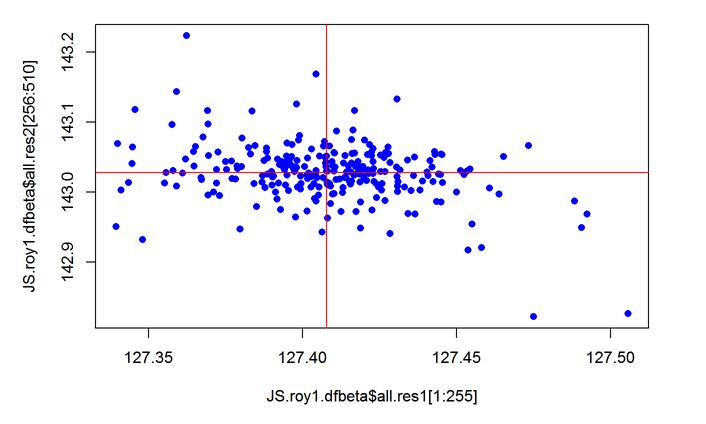
\includegraphics[width=0.7\linewidth]{images/dfbetas-JS-ROY}
	\caption{}
	\label{fig:dfbetas-JS-ROY}
\end{figure}






%---------------------------------------------------------------------------%
\newpage
\section{Likelihood Distance} %1.11
The \index{likelihood distance} likelihood distance is a global, summary measure, expressing the joint influence of the observations in the set $U$ on all parameters in $\phi$  that were subject to updating. 


The likelihood distance gives the amount by which the log-likelihood of the full data changes if one were
to evaluate it at the reduced-data estimates. The important point is that $l(\psi_{(U)})$ is not the log-likelihood
obtained by fitting the model to the reduced data set.

It is obtained by evaluating the likelihood function based on the full data set (containing all n observations) at the reduced-data estimates.




%
%
%%---------------------------------------------------------- %
%%Likelihood Displacement.
%\[  LD(\boldsymbol{(U)})= 2[l\boldsymbol{\hat{(\phi)}} - l\boldsymbol{\hat{\phi}_\omega} ] \]
%\[  RLD(\boldsymbol{(U)})= 2[ l_R\boldsymbol{\hat{(\phi)}} - l_R\boldsymbol{\hat{(\phi)}_\omega} ] \]
%%	Large values indicate that $\boldsymbol{\hat{\theta}}$ and $\boldsymbol{\hat{\theta}_\omega}$ differ considerably.


%========================================================= %
%- D
\newpage
\subsection*{4. Using DFBETAs to Assess Agreement}
Suppose an LME model was formulated to model agreement for various (i.e. 2 or more) methods of measurement, with replicate measurements. If the methods are to be agreement, the DFBetas for each case would be the same for both methods.\textbf{As such, agreement between any two methods can be determined by a simple scatterplot of the DFBetas. If the points align along the line of equality, then both methods can be said to be in agreement.}

%Cook's Distance can be used to identify and rank cases, in terms of influence.
For the model fitted to the blood data with the lme4 R package, the results tabulated below can be produced. All 85 subjects are ranked by Cook's Distance (with only the top 6 being presented here). The remaining columns are the DFBeta for each of the fixed effects, for each of the 85 subject.
\begin{center}
	\begin{tabular}{|c|c|c|c|c|} \hline
		Subject &    Cook's D  &    methodJ  &   methodR  & methodS \\ \hline \hline
		78 & 0.61557407 & -0.02934556 & -0.03387780 & 0.2954937  \\ \hline
		80 & 0.41590973 & -0.06305026 & -0.06515241 & 0.2123881  \\ \hline
		68 & 0.22536651 & -0.05334867 & -0.05062375 & 0.1555187  \\ \hline
		72 & 0.09348500  & 0.02388626  & 0.02419887 & 0.1617474  \\ \hline
		48 & 0.08706988  & 0.02147541  & 0.03145273 & 0.1581591  \\ \hline
		30 & 0.07118415  & 0.26925807  & 0.26215970 & 0.1581569  \\ \hline
	\end{tabular} 
\end{center}
\newpage
\begin{figure}[h!]
	\centering
	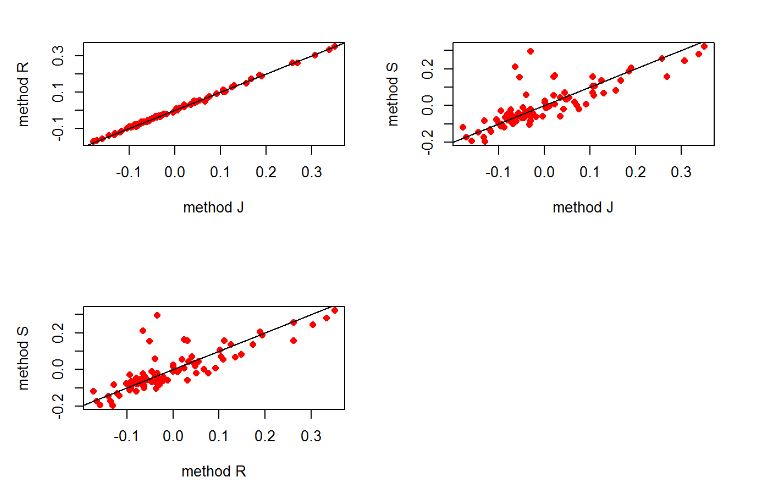
\includegraphics[width=0.9\linewidth]{images/04-DFbetaplots}
	% \caption{}
	% \label{fig:04-DFbetaplots}
\end{figure}

In the first of the three plots (\textit{Top Right}), strong agreement between method J and method R is indicated. The other plots indicate lack of agreement of methods J and R with method S.



If lack of agreement is indicated, a subsequent analysis using a technique proposed by Roy(2009) can be used to identify the specific cause for this lack of agreement (see next section).
\newpage

The Pearson Correlation coefficient of the DFBetas can be used in conjection with this analysis. A high correlation confirms good agreement. No threshold value for agreement is suggested, and analysts are advised to perform model diagnostics regardless of the correlation coeffient. 


The Bonferroni Outlier Test and Cook's Distance values can be used to identify unusual cases, when the relationship between sets of dfbeta is modelled as a (classical) linear model. In this model, the covariates should be homoskedastic. A test for non-constant variance may be used to verify this. These diagnostic procedures are implementable using the \textbf{\textit{car}} R package.


Deming Regression can be used to verify the line of equality. Significance test for Deming regression estimates are not available, but 95\% bootstrap confidence intervals for the slope estimate and intercept estimates can be computed. 


Additionally a mean difference plot can be used to identify outliers. This mean-difference plot differs from the Bland-Altman plot in that the plot is denominated in terms of dfbeta values, and not in measurement units.

If lack of agreement is indicated between methods of measurement, use of Roy's Testing is advised (This is the subject of the next section).
\begin{figure}[h1]
	\centering
	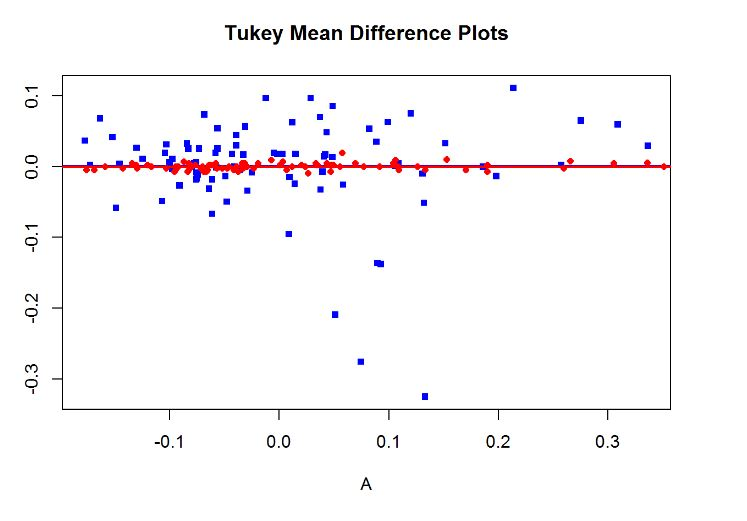
\includegraphics[width=0.7\linewidth]{images/04-TMDplot}

\end{figure}
\newpage
%========================================================= %
%% - Part E
\subsection*{5. Using Roy's Test to Identify cause of Lack of agreement}

Barnhart specifies three conditions for method of measurement that are required for two methods of measurement to be considered in agreement.

\begin{itemize}
	\item[(i)] No Significant Inter-method bias
	\item[(ii)] No significant Difference in Within-Subject Variance
	\item[(iii)] No significant Difference in Within-Subject Variance 
\end{itemize}


Roy(2009) demonstrates a LME model specification, and a series of tests that look at each of these agreement criteria individually. If two methods of measuement lack agreement, the specific reason or reasons for this lack of agreement can be identified.


Roy proposes an LME model with Kronecker product covariance structure in a doubly multivariate setup. Response for $i$th subject can be written as
\[ y_i = \beta_0 + \beta_1x_{i1} + \beta_2x_{i2} + b_{1i}z_{i1}  + b_{2i}z_{i2} + \epsilon_i \]
\begin{itemize}
	\item $\beta_1$ and $\beta_2$ are fixed effects corresponding to both methods. ($\beta_0$ is the intercept.)
	\item $b_{1i}$ and $b_{2i}$ are random effects corresponding to both methods.
\end{itemize}

Overall variability between the two methods ($\Omega$) is sum of between-subject ($D$) and within-subject variability ($\Sigma$),
\[
\mbox{Block } \boldsymbol{\Omega}_i = \left[ \begin{array}{cc} d^2_1 & d_{12}\\ d_{12} & d^2_2\\ \end{array} \right]
+ \left[\begin{array}{cc} \sigma^2_1 & \sigma_{12}\\ \sigma_{12} & \sigma^2_2\\ \end{array}\right].
\]
%============================================== %
%- F:
\subsection*{6. Using Roy's Model to Compute LoAs and CR }

In this short section, a demonstration of how Roy's technique can be used to compute two common MCS metrics: Limits of Agreement and the Coefficient of Repeatabilty. While Limits of Agreement are not used in the analysis proposed here, they are ubiquituous in literature, and a demonstration on how to compute them with the Roy Model would assist the adoption of this proposed method.

The coefficient of repeatability is encountered in Gage R \& R analysis. \textit{(A future exploration of how LME models can be used in that field would be of interest. This is something to include in the Conclusions Section).}
%============================================== %
%- G:
\subsection*{7. Model Diagnostics for Roy's Models}

Further to previous work, this section revisits case-deletion and residual diagnostics, and explores how approaches devised by  Galecki \& Burzykowski (2013) can be used to appraise Roy's model. These authors specifically look at Cook's Distances and Likelihood Distances.
For the Roy Model, Cook's Distances may also be generated using the \textbf{\textit{predictmeans}}



\begin{figure}[h!]
	\centering
	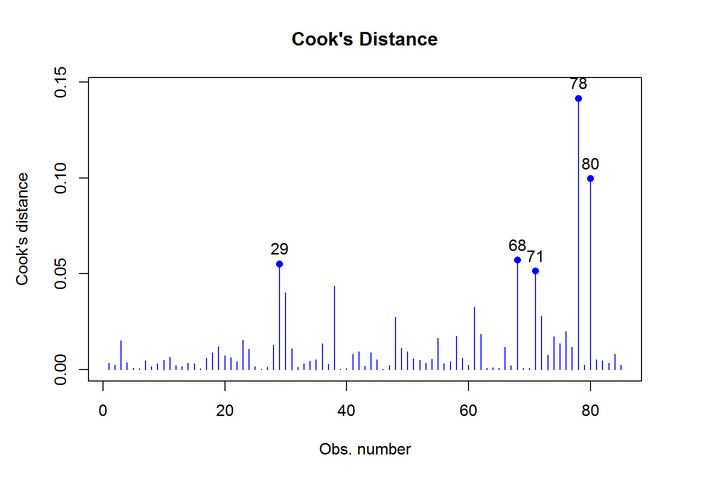
\includegraphics[width=0.7\linewidth]{images/CooksDistancePlot-JS-Roy}
	\caption{}
	\label{fig:CooksDistancePlot-JS-Roy}
\end{figure}

\begin{figure}[h!]
	\centering
	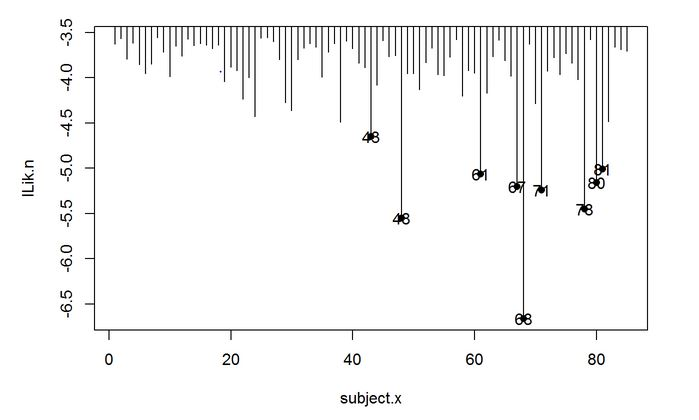
\includegraphics[width=0.7\linewidth]{images/LogLik-JS-Roy}
	\caption{}
	\label{fig:LogLik-JS-Roy}
\end{figure}

As the model is structurally different from the models discussed in the earlier sections, Residual analysis will be briefly revisited.
\begin{figure}[h!]
	\centering
	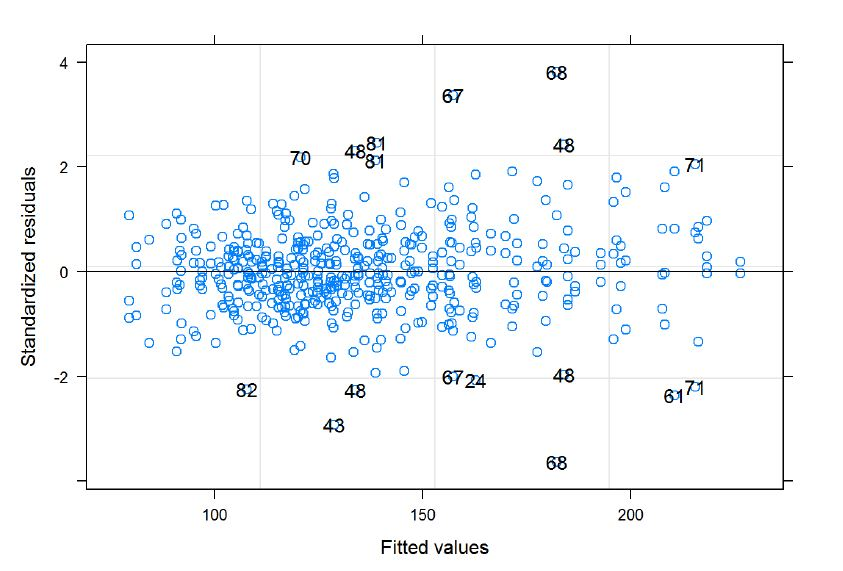
\includegraphics[width=0.7\linewidth]{images/Residuals-JS-Roy}
	\caption{}
	\label{fig:Residuals-JS-Roy}
\end{figure}

\newpage
\subsection*{8. Case Deletion Diagnostics for the Variance Ratios}
%- H Case Deletion Diagnostics 

Schabenberger advises on the use of deletion diagnostics for variance components of an LME model.
Taking the core principals of his methods, and applying them to the Method Comparison problem, case deletion diagnostics are used on the variance components of the Roy model., specifically the ratio of between subject variances and the within subject covariances respecitvely.


\[ \mbox{BSVR} = \frac{\sigma^2_2}{\sigma^2_2} \phantom{makespace}  \mbox{WSVR} = \frac{d^2_2}{d^2_2} \]

These variance ratios are re-computed for each case removed, and may be analysed seperately or jointly for outliers. 

The Grubbs' Test for Outliers is a commonly used technique for assessing outlier in a univariate data set. As there may be several outliers (i.e. influential cases) present, the Grubbs test is not practical. However outlier detection using to Tukey's 
specification for boxplots (i.e. greater than $Q_3 +1.5 IQR$ or less than $Q_1 - 1.5 IQR$), will suffice. Ranking the asbolute values of the standardizaed scores can also can be used to identify influential cases, even if the data is not normally distributed.

Bivariate Analyses may be applied jointly to the both sets of data sets, e.g Mahalanobis distances. The Mahalanobis distance, while not an intuitive measure in the context of the data, can be used to rank highly influential cases. 

%============================================== %
% - I: 
\subsection*{9. Permutation Test, Power Tests and Missing Data }

This section explores topics such as dependent variable simulation and power analysis, introduced by Galecki \& Burzykowski (2013), and implementable with their \textbf{\textit{nlmeU}} \texttt{R} package.
Using the \textbf{\textit{predictmeans}} \texttt{R} package, it is possible to perform permutation t-tests for coefficients of (fixed) effects and permutation F-tests.

The matter of missing data has not been commonly encountered in either Method Comparison Studies or Linear Mixed Effects Modelling. However Roy (2009) deals with the relevant assumptions regrading missing data. Galecki \& Burzykowski (2013) approaches the subject of missing data in LME Modelling. The \textbf{\textit{nlmeU}} package includes the \texttt{patMiss} function, which ``\textit{allows to compactly present pattern of missing data in a given vector/matrix/data
	frame or combination of thereof}".


%================================================%

%-------------------------------------------------------------------------------------------------------------------------------------%
\subsection{Influential Observations : DFBeta and DFBetas}
\section{Measures of Influence} %1.16

The impact of an observation, or a case with multiple obverations, on a regression fitting can be determined by the difference between the estimated regression coefficient of a model with all observations and the estimated coefficient when the particular observation is deleted. The measure DFBETA is the studentized value of this difference.


\section{Overall Influence}
An overall influence statistic measures the change in the objective function being minimized. For example, in
OLS regression, the residual sums of squares serves that purpose. In linear mixed models fit by
\index{maximum likelihood} maximum likelihood (ML) or \index{restricted maximum likelihood} restricted maximum likelihood (REML), an overall influence measure is the \index{likelihood distance} likelihood distance [Cook and Weisberg ].
%============================================================================= %

\section{Effects on fitted and predicted values}
\begin{equation}
	\hat{e_{i}}_{(U)} = y_{i} - x\hat{\beta}_{(U)}
\end{equation}




%============================================================================= %
\section{Cooks's Distance}
Cook's Distance is a measure indicating to what extent model parameters are influenced by (a set of) influential data on which the model is based. This function computes the Cook's distance based on the information returned by the estex() function.
	%---------------------------------------------------------------------------%
	
	\subsection{Cook's Distance}
	\begin{itemize}
		\item For variance components $\gamma$: $CD(\gamma)_i$,
		\item For fixed effect parameters $\beta$: $CD(\beta)_i$,
		\item For random effect parameters $\boldsymbol{u}$: $CD(u)_i$,
		\item For linear functions of $\hat{beta}$: $CD(\psi)_i$
	\end{itemize}
	
	\newpage
	\subsubsection{Random Effects}
	
	A large value for $CD(u)_i$ indicates that the $i-$th observation is influential in predicting random effects.
	
	\subsubsection{linear functions}
	
	$CD(\psi)_i$ does not have to be calculated unless $CD(\beta)_i$ is large.
	
	
	%	\subsection{Information Ratio}
	%	
	%	\newpage
	%	\section*{Cook's Distance} %1.9
	%	
	%Cook (1977)
	\textit{Cook (1977)} greatly expanded the study of residuals and influence measures. Cook's key observation was the effects of deleting each observation in turn could be computed without undue additional computational expense. Consequently deletion diagnostics have become an integral part of assessing linear models.
	
	
	Cook (1986) gave a completely general method for assessing influence of local departures from
	assumptions in statistical models.
	
	
	\subsection{Cook's Distance}%1.9.3
	\index{Cook's Distance}
	In classical linear regression, a commonly used meausre of influence is Cook's distance. It is used as a measure of influence on the regression coefficients.
	
	For linear mixed effects models, Cook's distance can be extended to model influence diagnostics by definining.
	
	\[ C_{\beta i} = {(\hat{\beta} - \hat{\beta}_{[i]})^{T}(\boldsymbol{X}^{\prime}\boldsymbol{V}^{-1}\boldsymbol{X}) (\hat{\beta} - \hat{\beta}_{[i]}) \over p}\]
	
	It is also desirable to measure the influence of the case deletions on the covariance matrix of $\hat{\beta}$.
	
	
	
	
	

	
		\subsection{Cooks's Distance}%1.9.2
		\index{Cook's distance} Cook's $D$ statistics (i.e. colloquially Cook's Distance) is a measure of the influence of observations in subset $U$ on a vector of parameter estimates \citep{cook77}.
		
		\[ \delta_{(U)} = \hat{\beta} - \hat{\beta}_{(U)}\]
		
		If V is known, Cook's D can be calibrated according to a chi-square distribution with degrees of freedom equal to the rank of $\boldsymbol{X}$ \citep{cpj92}.
		
	
	For LME models, Cook's distance can be extended to model influence diagnostics by defining.
	
	%\[ C_{\beta i} = {(\hat{\beta} - \hat{\beta}_{[i]})^{T}(\boldsymbol{X}^{\prime}\boldsymbol{V}^{-1}\boldsymbol{X}) (\hat{\beta} - \hat{\beta}_{[i]}) \over p}\]
	
	It is also desirable to measure the influence of the case deletions on the covariance matrix of $\hat{\beta}$.
	
	\section{Cook's Distance for LMEs} %1.10
	Diagnostic methods for fixed effects are generally analogues of methods used in classical linear models.
	Diagnostic methods for variance components are based on `one-step' methods. Cook (1986) gives a completely general method for assessing the influence of local departures from assumptions in statistical models.
	
	For fixed effects parameter estimates in LME models, the \index{Cook's distance} Cook's distance can be extended to measure influence on these fixed effects.
	
	\[
	\mbox{CD}_{i}(\beta) = \frac{(c_{ii} - r_{ii}) \times t^2_{i}}{r_{ii} \times p}
	\]
	
	For random effect estimates, the \index{Cook's distance} Cook's distance is
	
	\[
	\mbox{CD}_{i}(b) = g{\prime}_{(i)} (I_{r} + \mbox{var}(\hat{b})D)^{-2}\mbox{var}(\hat{b})g_{(i)}.
	\]
	Large values for Cook's distance indicate observations for special attention.
	
	
	\subsection*{Cook's Distance}%1.19.1 
	Cooks Distance ($D_{i}$) is an overall measure of the combined impact of the $i$th case of all estimated regression coefficients. It uses the same structure for measuring the combined impact of the differences in the estimated regression coefficients when the $i-$th case is deleted.
	
	Importantly, $D_{(i)}$ can be calculated without fitting a new regression coefficient each time an observation is deleted.
	

	
	
	Cook (1977) greatly expanded the study of residuals and influence measures. Cook's key observation was the effects of deleting each observation in turn could be computed without undue additional computational expense. Consequently deletion diagnostics have become an integral part of assessing linear models.
	
	
	\index{Cook's distance}Cook's Distance is a well known diagnostic technique used in classical linear models, extended to LME models.  For LME models, two formulations exist; a \index{Cook's distance}Cook's distance that examines the change in fixed fixed parameter estimates, and another that examines the change in random effects parameter estimates. The outcome of either Cook's distance is a scaled change in either $\beta$ or $\theta$.
	
	
	\subsection{Cook's Distance}
	In statistics, Cook's Distance or Cook's D is a commonly used estimate of the influence of a data point when performing least squares regression analysis.[1] In a practical ordinary least squares analysis, Cook's distance can be used in several ways: to indicate data points that are particularly worth checking for validity; to indicate regions of the design space where it would be good to be able to obtain more data points. It is named after the American statistician R. Dennis Cook, who introduced the concept in 1977.
		

	
	\subsection{Change in the precision of estimates}
	
	The effect on the precision of estimates is separate from the effect on the point estimates. Data points that
	have a small \index{Cook's distance}Cook's distance, for example, can still greatly affect hypothesis tests and confidence intervals, if their  influence on the precision of the estimates is large.
	
	


	
	
	\subsubsection{Interpretation}
	Specifically $D_i$ can be interpreted as the distance one's estimates move within the confidence ellipsoid that represents a region of plausible values for the parameters.[clarification needed] This is shown by an alternative but equivalent representation of Cook's distance in terms of changes to the estimates of the regression parameters between the cases where the particular observation is either included or excluded from the regression analysis.
	

	
	
	\subsection{Cook's Distance}
	% Interpretation
	% http://stats.stackexchange.com/questions/22161/how-to-read-cooks-distance-plots %
	Some texts tell you that points for which Cook's distance is higher than 1 are to be considered as influential. Other texts give you a threshold of $4/N$ or $4/(N−k−1)$, where N is the number of observations and k the number of explanatory variables. In your case the latter formula should yield a threshold around 0.1 .
	
	John Fox (1), in his booklet on regression diagnostics is rather cautious when it comes to giving numerical thresholds. He advises the use of graphics and to examine in closer details the points with "values of D that are substantially larger than the rest". According to Fox, thresholds should just be used to enhance graphical displays.
	
	In your case the observations 7 and 16 could be considered as influential. Well, I would at least have a closer look at them. The observation 29 is not substantially different from a couple of other observations.
	
	(1) Fox, John. (1991). Regression Diagnostics: An Introduction. Sage Publications.
	%============================================================================= %
\chapter{Appendices 1}


\section{Model Terms (Roy 2009)}
\begin{itemize}
	\item Let $y_{mir}$ be the response of method $m$ on the $i$th subject
	at the $r-$th replicate.
	\item Let $\boldsymbol{y}_{ir}$ be the $2 \times 1$ vector of measurements
	corresponding to the $i-$th subject at the $r-$th replicate.
	\item Let $\boldsymbol{y}_{i}$ be the $R_i \times 1$ vector of
	measurements corresponding to the $i-$th subject, where $R_i$ is number of replicate measurements taken on item $i$.
	\item Let $\alpha_mi$ be the fixed effect parameter for method for subject $i$.
	\item Formally Roy uses a separate fixed effect parameter to describe the true value $\mu_i$, but later combines it with the other fixed effects when implementing the model.
	\item Let $u_{1i}$ and $u_{2i}$ be the random effects corresponding to methods for item $i$.
	
	\item $\boldsymbol{\epsilon}_{i}$ is a $n_{i}$-dimensional vector
	comprised of residual components. For the blood pressure data $n_{i} = 85$.
	
	\item $\boldsymbol{\beta}$ is the solutions of the means of the two methods. In the LME output, the bias ad corresponding
	t-value and p-values are presented. This is relevant to Roy's first test.\end{itemize}





%------------------------------------------------%
\newpage

\section{Algorithms : ML v REML}
Maximum likelihood estimation is a method of obtaining estimates of unknown parameters by optimizing a likelihood function. The ML
parameter estimates are the values of the argument that maximise the likelihood function, i.e. the estimates that make the observed
values of the dependent variable most likely, given the distributional assumptions

The most common iterative algorithms used for the optimization
problem in the context of LMEs are the EM algoritm, fisher scoring
algorithm and NR algorithm, which [cite:West] commends as the
preferred method.

A mixed model is an extension of the general linear models that
can specify additional random effects terms.

Parameter of the mixed model can be estimated using either ML or
REML, while the AIC and the BIC can be used as measures of
"goodness of fit" for particular models, where smaller values are
considered preferable.

%--------------------------------------------------------------------%

(\textbf{\emph{Wikipedia}})The restricted (or residual, or reduced) maximum likelihood (REML) approach is a particular form of maximum likelihood estimation which does not base estimates on a maximum likelihood fit of all the information, but instead uses a likelihood function calculated from a transformed set of data, so that nuisance parameters have no effect.

In contrast to the earlier maximum likelihood estimation, REML can produce unbiased estimates of variance and covariance parameters.

%-----------------------------------------------------------------------------------------%

\noindent \textbf{ML procedures for LME}

The maximum likelihood procedure of Hartley and Rao yields
simultaneous estimates for both the fixed effects and the random
effect, by maximising the likelihood of $\boldsymbol{y}$ with
respect to each element of $\boldsymbol{\beta}$ and
$\boldsymbol{b}$.

%-----------------------------------------------------------------------------------------%
\newpage
\section{Estimation of random effects}

Estimation of random effects for LME models in the NLME package is accomplished through use
of both EM (Expectation-Maximization) algorithms and Newton-Raphson algorithms.
\begin{itemize}
	\item EM iterations bring estimates of the parameters into the region of the optimum very quickly, but
	convergence to the optimum is slow when near the optimum.
	\item Newton-Raphson iterations are computationally intensive and can be unstable when far from the
	optimum. However, close to the optimum they converge quickly.
	\item The LME function implements a hybrid approach, using 25 EM iterations to quickly get near the
	optimum, then switching to Newton-Raphson iterations to quickly converge to the optimum. \item If
	convergence problems occur, the ``control�argument in LME can be used to change the way the
	model arrives at the optimum.
\end{itemize}

	
	
	
	%--Marginal and Conditional Residuals
	
	
	\section{Covariance Parameters} %1.5
	The unknown variance elements are referred to as the covariance parameters and collected in the vector $\theta$.
	% - where is this coming from?
	% - where is it used again?
	% - Has this got anything to do with CovTrace etc?
	%---------------------------------------------------------------------------%
	
	\subsection{Methods and Measures}
	The key to making deletion diagnostics useable is the development of efficient computational formulas, allowing one to obtain the \index{case deletion diagnostics} case deletion diagnostics by making use of basic building blocks, computed only once for the full model.
	
	\citet{Zewotir} lists several established methods of analyzing influence in LME models. These methods include \begin{itemize}
		\item Cook's distance for LME models,
		\item \index{likelihood distance} likelihood distance,
		\item the variance (information) ration,
		\item the \index{Cook-Weisberg statistic} Cook-Weisberg statistic,
		\item the \index{Andrews-Prebigon statistic} Andrews-Prebigon statistic.
	\end{itemize}
%--------------------------------------------------------------------------------------------%
%--------------------------------------------------------------------------------------------%
	\newpage
	\section{Computation and Notation } %2.3
	with $\boldsymbol{V}$ unknown, a standard practice for estimating $\boldsymbol{X \beta}$ is the estime the variance components $\sigma^2_j$,
	compute an estimate for $\boldsymbol{V}$ and then compute the projector matrix $A$, $\boldsymbol{X \hat{\beta}}  = \boldsymbol{AY}$.
	
	
	\citet{Zewotir} remarks that $\boldsymbol{D}$ is a block diagonal with the $i-$th block being $u \boldsymbol{I}$
	%--------------------------------------------------------------%
	\newpage
	\section{Measures 2} %2.4
	
	\subsection{Cook's Distance} %2.4.1
	\begin{itemize}
		\item For variance components $\gamma$
	\end{itemize}
	
	Diagnostic tool for variance components
	\[ C_{\theta i} =(\hat(\theta)_{[i]} - \hat(\theta))^{T}\mbox{cov}( \hat(\theta))^{-1}(\hat(\theta)_{[i]} - \hat(\theta))\]
	\newpage
	\section{Haslett's Analysis} %2.5
	For fixed effect linear models with correlated error structure Haslett (1999) showed that the effects on
	the fixed effects estimate of deleting each observation in turn could be cheaply computed from the fixed effects model predicted residuals.

	
	
	%-------------------------------------------------------------------------------------------------------%
	\chapter{Appendices} % Chapter 5
	%---------------------------------------------------------------------------------------------------------%
	% Appendices
	% - The Hat Matrix (5.1)
	% - Sherman Morrison Woodbury Formula (5.2)
	% -  Hat Matrix applied to MCS (5.3)
	% - Cross Validation (Updating standard deviation) (5.4)
	% - Updating Estimates (5.5)
	% - Lesaffre's paper (5.6)
	%---------------------------------------------------------------------------------------------------------%
	%------------------------------------------------------------------------%

	
	\newpage
	\section{Measures 2} %2.4
	
	\subsection{Cook's Distance} %2.4.1
	\begin{itemize}
		\item For variance components $\gamma$
	\end{itemize}
	
	Diagnostic tool for variance components
	\[ C_{\theta i} =(\hat(\theta)_{[i]} - \hat(\theta))^{T}\mbox{cov}( \hat(\theta))^{-1}(\hat(\theta)_{[i]} - \hat(\theta))\]
	
	\subsection{Variance Ratio} %2.4.2
	\begin{itemize}
		\item For fixed effect parameters $\beta$.
	\end{itemize}
	
	\subsection{Cook-Weisberg statistic} %2.4.3
	\begin{itemize}
		\item For fixed effect parameters $\beta$.
	\end{itemize}
	
	\subsection{Andrews-Pregibon statistic} %2.4.4
	\begin{itemize}
		\item For fixed effect parameters $\beta$.
	\end{itemize}
	The Andrews-Pregibon statistic $AP_{i}$ is a measure of influence based on the volume of the confidence ellipsoid.
	The larger this statistic is for observation $i$, the stronger the influence that observation will have on the model fit.
	
	
	%---------------------------------------------------------------------------%
	
	
	\section{Computation and Notation } %2.3
	with $\boldsymbol{V}$ unknown, a standard practice for estimating $\boldsymbol{X \beta}$ is the estime the variance components $\sigma^2_j$,
	compute an estimate for $\boldsymbol{V}$ and then compute the projector matrix $A$, $\boldsymbol{X \hat{\beta}}  = \boldsymbol{AY}$.
	
	
	\citet{Zewotir} remarks that $\boldsymbol{D}$ is a block diagonal with the $i-$th block being $u \boldsymbol{I}$
	%--------------------------------------------------------------%
	\newpage
	\section{Measures 2} %2.4
	
	\subsection{Cook's Distance} %2.4.1
	\begin{itemize}
		\item For variance components $\gamma$
	\end{itemize}
	
	Diagnostic tool for variance components
	\[ C_{\theta i} =(\hat(\theta)_{[i]} - \hat(\theta))^{T}\mbox{cov}( \hat(\theta))^{-1}(\hat(\theta)_{[i]} - \hat(\theta))\]
	
	\subsection{Variance Ratio} %2.4.2
	\begin{itemize}
		\item For fixed effect parameters $\beta$.
	\end{itemize}
	
	\subsection{Cook-Weisberg statistic} %2.4.3
	\begin{itemize}
		\item For fixed effect parameters $\beta$.
	\end{itemize}
	
	\subsection{Andrews-Pregibon statistic} %2.4.4
	\begin{itemize}
		\item For fixed effect parameters $\beta$.
	\end{itemize}
	The Andrews-Pregibon statistic $AP_{i}$ is a measure of influence based on the volume of the confidence ellipsoid.
	The larger this statistic is for observation $i$, the stronger the influence that observation will have on the model fit.
	\newpage
\bibliographystyle{chicago}
\bibliography{DB-txfrbib}
\end{document}

%---------------------------------------------------------------------------------------------------%


